

The description of the model follows the ODD (Overview, Design concepts, Details) protocol for IBMs \citep{Grimm2006ODD,Grimm2010UpdateODD,Grimm2020SecondUpdateODD}. The IBM is implemented in Python 3.7, and is available in the electronic supplementary material.

\subsection{Purpose and Patterns}\label{sec:purpose}

 The first purpose of this model is to predict the number, location, size spectrum and population dynamics of shelled pteropods in response to the heterogeneous environmental conditions in the CalCS. Ultimately, the purpose of this model, which will be presented in follow-up work, is to explore the relationship between pteropod populations and environmental stressors such as acidification. To this end, we impose a fixed life cycle with two generations for temperate pteropods \citep{Wang2017Lifecycle} and developmental timings of life stages and key traits and behaviours \citep[e.g. protoconch, parapodia, onset of diel vertical migration, and maturity; ][]{Howes2014Lab,Thabet2015Lifestages} as a function of shell size to simulate population dynamics. The impacts of stressors are implemented to reduce shell size growth, which allows our model to simulate the impacts of stressors on the life history, behaviour, population demographics and spatio-temporal distribution of individual pteropods.
 

 
 
%  quantify and characterize  the sublethal effects of changing ocean chemistry on populations of shelled pteropods. The model characterizes the role of the different life stages, life history and behavior in relation to the population-level response to changes in ocean chemistry. The model is based on laboratory data for \textit{L. helicina}, and \textit{L. retroversa} or in-situ observations of shelled pteropods in the temperate regions.
 
%  We evaluate our model by its ability to reproduce observed abundance patterns.  Although sublethal effects of changes in ocean chemistry have been recorded on an individual level \citep{Bednarsek2017ExposureHistory}, traditional population-level analyses have not detected significant changes in the abundance of pteropods \citep{Ohman2009Multi}. Thus, bulk measures such as abundance, and the timing of abundance peaks should be reproduced in our model despite the sublethal effects on on an individual-level.
 

\subsection{Entities, state variables, and scales}\label{sec:entities}

Our model includes one entity, the shelled pteropods. The pteropods are characterized by twelve state variables (Tab. \ref{tab:state_variables_pteropods}), such as the ID, the parent ID, parent size during spawning, generation, age, size, Egg Release Readiness (ERR) index, spawning events, undersaturation experienced, accumulated damage, date and location. 
The ID and parent ID are unique identifiers for each pteropod and the pteropod that spawned them. The parent size represents the shell length ($mm$) of the parent pteropod during spawning. The generation is an integer used to differentiate between pteropods of the spring (even integer) and overwintering (odd integer) generation as described for temperate regions \citep{Dadon1992Reproduction,lalli1989pelagic,Wang2017Lifecycle,Maas2020Lipids}. The life time of pteropods is measured using the age attribute in days since spawning. The current shell size is given by the size attribute ($mm$). The Egg Release Readiness (ERR) index \citep[similar to the Clutch Readiness Fraction presented in ][]{Miller1998CalanusIBM} represents whether a mature pteropod is ready to spawn eggs or not. The spawning events represents the number of times a pteropod has produced and released eggs. The undersaturation experienced ($\Omega_{arag}$) quantifies the average $\Omega_{arag}$ experienced by a pteropod in one day. The accumulated damage quantifies the amount of CaCO$_3$ ($mg$) lost due to dissolution throughout the life each pteropod after calcification/repair. The date and location depict the day in a year, and the depth ($m$), latitude ($\degree N$) and longitude ($\degree E$) of the pteropod. The location and date attributes enable us to analyze the IBM using a circulation model output. However, the IBM on its own does not have a spatial scale. The IBM's total simulation time is not constrained, and is run at a one-day time step.

\begin{table}[h!]
    
    \caption{Summary of state variables characterizing the simulated shelled pteropods.}
    \label{tab:state_variables_pteropods}
    \centering
    \scriptsize
    \begin{tabulary}{0.9\textwidth}{LLL}
    
    
        \hline
        \textbf{Variable name}                & \textbf{Variable type and units}                       & \textbf{Meaning}                                             \\ \hline
        ID                                    & Static integer without units                           & Unique identifier for each pteropod                          \\ \hline
        Parent ID                             & Static integer without units                           & Unique identifier of the parent pteropod                     \\ \hline
        Parent size                           & Static real number in $mm$                      & Shell size of the parent pteropod at the time of spawning    \\ \hline
        Generation          & Static integer without units      & Integer used to identify whether a pteropod corresponds to the spring (even integer) or overwintering (odd integer) generation \\ \hline
        Age                      & Dynamic integer in days since birth                         & Number of days passed since the pteropod was spawned         \\ \hline
        Size                                  & Dynamic real number in $mm$                     & Shell size or length of the pteropod                         \\ \hline
        
        Egg Release Readiness (ERR) index           & Dynamic real number between 0.0 and 1.0 without units  & Fraction depicting whether a pteropod is ready to spawn eggs. Spawning only begins if $ERR \geq 1.0$.  \\ \hline
        Spawning events & Dynamic integer without units & Describes the number of times a pteropod has produced and released eggs. \\ \hline
        Undersaturation experienced ($\Omega_{arag}$)   & Dynamic real number without units & Average $\Omega_{arag}$ experienced by a pteropod in one day \\ \hline
        Accumulated damage & Dynamic real number in $mg$ CaCO$_3$ & Net amount of CaCO$_3$ lost due to dissolution throughout the life of a pteropod \\ \hline
        Date      & Dynamic integer for the date & Current date          \\ \hline
        Location    & Dynamic real numbers in $m$, $\degree$N and $\degree$E & Location of the pteropod given in depth, latitude and longitude \\ \hline
    \end{tabulary}
\end{table}



\subsection{Process overview and scheduling}\label{sec:process_overview}
In this section we provide an overview of the processes that occur in our IBM, the order in which they are executed, and focus on how the state variables are changed. Out of the twelve state variables, the age, size, ERR index, spawning events, $\Omega_{arag}$, accumulated damage, date and location are changed on each one-day time step by the following five processes (Fig. \ref{fig:flow_chart}): (1) Movement and $\Omega_{arag}$ tracker, (2) Mortality, (3) Shell growth, (4) Development, (5) Spawning eggs.
\begin{enumerate}
    \item \textit{Movement and $\Omega_{arag}$ tracker}: This function computes the vertical and horizontal movement of pteropods and tracks the $\Omega_{arag}$ that pteropods experience on a one-hour time step at each location. The higher temporal resolution was chosen, since vertical migration can result in exposure to corrosive and non-corrosive waters within a day \citep{Bednarsek2015VerticalDistribution}. In order to fit the simulation time step of one day, we calculate the average $\Omega_{arag}$ experienced by each pteropods in a 24 hour window. The movement and tracking of $\Omega_{arag}$ was calculated using the Lagrangian ocean analysis tool Parcels v2.1.3 \citep{Delandmeter2019Unbeaching}. This Lagrangian tool uses custom Parcels objects for the execution, and thus we have to translate the information for each pteropod stored as a numpy array \citep{oliphant2006guide} into the custom Parcels object back and forth before and after the execution of the \textit{Movement and $\Omega_{arag}$ tracker} function. 
    \item \textit{Mortality}: This function computes whether a pteropod dies or continues to live based on daily size-dependent mortality rates, the age of the pteropods, generation, and number of spawning events. 
    \item \textit{Shell growth}:  This function determines the net shell growth, i.e. growth, including dissolution and repair, given the daily average $\Omega_{arag}$ exposure calculated in \textit{Movement and $\Omega_{arag}$ tracker}.
    \item \textit{Development}: This function determines the life stage that each pteropod has reached based on their size. Different life stages are linked to the development of key traits/organs (e.g. protoconch, parapodia, juvenile/adult shell, maturity). These key traits/organs are used in other functions, e.g. the development of the protoconch and parapodia to mark the onset of shell dissolution and DVM, respectively.
   \item \textit{Spawning}: This function determines whether a pteropod has reached maturity and is ready to spawn eggs.
\end{enumerate}

% \subsubsection{Movement and $\Omega_{arag}$ tracker}

% The \textit{Movement and $\Omega_{arag}$ tracker} function (Fig. \ref{fig:flow_chart}) computes the vertical and horizontal movement of pteropods and tracks the $\Omega_{arag}$ that pteropods experience at at a one-hour time step in each location. The higher temporal resolution was chosen, since vertical migration can result in exposure to corrosive and non-corrosive waters within a day \citep{Bednarsek2015VerticalDistribution}. In order to fit the simulation time step of one day, we calculate the average $\Omega_{arag}$ experienced by each pteropods in a 24 hour window. The movement and tracking of $\Omega_{arag}$ was calculated using the Lagrangian ocean analysis tool Parcels v2.1.3 \citep{Delandmeter2019Unbeaching}. This Lagrangian tool uses custom Parcels objects for the execution, and thus we have to translate the information for each pteropod stored as a numpy array \citep{oliphant2006guide} into the custom Parcels object back and forth before and after the execution of the \textit{Movement and $\Omega_{arag}$ tracker} function. 

% \subsubsection{Mortality}
% The function \textit{Mortality} computes whether a pteropod dies or continues to live using size-dependent daily mortality rates. 


% Pteropods that survive execute the function \textit{Shell growth}, which determines the net shell growth (growth, including dissolution and repair) given the daily average $\Omega_{arag}$. Next, in the \textit{Develop} function pteropods that reach a certain size develop key traits/organs (e.g. protoconch, parapodia, juvenile/adult shell, maturity). If a pteropod reached maturity on the last time step, their ERR index is initialized to a random number between zero and one. For already mature pteropods, their ERR index increases by $\frac{1}{20}$ unless they spawned eggs in the previous time step. In the latter case, their ERR index is reset to zero. At the end of the function \textit{Develop}, the age of all pteropods is increased by one day. Finally, we search the current pteropod population for mature individuals with $ERR \geq 1.0$ in function \textit{Spawn eggs}. If such individuals are found, they spawn new pteropods.

% First, the function \textit{Prepare secondary attributes} is executed to calculate high level variables or secondary attributes derived from state variables such as generation, size, date and location attributes. High level variables include the life stage, days since maturity, upward and downward swimming velocities, the maximum depth that pteropods aim to reach during their downward migration, and the time at which pteropods start their downward and upward migration relative to the sunrise and sunset, respectively.





% The IBM covers two generations of shelled pteropods per year \citep[i.e. the spring and overwintering generation; ][]{Dadon1992Reproduction,lalli1989pelagic,Wang2017Lifecycle,Maas2020Lipids}. Pteropods experience different processes along their life time, such as the vertical migration \citep{Bednarsek2015VerticalDistribution}, shell repair \citep{Comeau2010RepairRates,Bednarsek2014CalcificationDissolution}, shell growth \citep{Wang2017Lifecycle}, and the development of key organs (protoconch, parapodia, juvenile/adult shell) \citep{Howes2014Lab,Thabet2015Lifestages}. These processes involve changes in high level variables that are calculated from the state variables generation, age, size, ERR index, date and location. Thus, in this section we provide an overview of the processes that occur in our IBM model, the order in which they are executed, and focus on how the state variables are changed. We provide this overview by naming the processes that occur in each time step, i.e. a simulation day, without the initialization steps (Fig. \ref{fig:flow_chart}). The full description of these processes, initialization steps, and description of high level variables is found in the appropriate sections \citep[section \ref{sec:initialization} and \ref{sec:submodels}; ][]{Grimm2006ODD,Grimm2010UpdateODD,Grimm2020SecondUpdateODD}.


% Out of the ten state variables of pteropods, the age, size, ERR index, $\Omega_{arag}$, date and location can be changed by processes along the life time of pteropods. On each time step six processes are executed in sequence:
% \begin{enumerate}
%     \item Prepare secondary attributes
%     \item Movement and $\Omega_{arag}$ tracker
%     \item Die off
%     \item Shell growth
%     \item Develop 
%     \item Spawn eggs
% \end{enumerate}
% First, the function \textit{Prepare secondary attributes} is executed to calculate high level variables or secondary attributes derived from state variables such as generation, size, date and location attributes. High level variables include the life stage, days since maturity, upward and downward swimming velocities, the maximum depth that pteropods aim to reach during their downward migration, and the time at which pteropods start their downward and upward migration relative to the sunrise and sunset, respectively. The \textit{Movement and $\Omega_{arag}$ tracker} function computes the vertical and horizontal movement of pteropods and tracks the $\Omega_{arag}$ that pteropods experience at each location using the Lagrangian ocean analysis tool Parcels v2.1.3 \citep{Delandmeter2019Unbeaching}. This Lagrangian tool uses custom objects for the execution, and thus the function \textit{Prepare secondary attributes} also translates the information for each pteropod stored as a numpy array \citep{oliphant2006guide} into the custom Parcels object. In general, the processes simulated in our IBM run at a one-day time step. However, vertical migration can results in the exposure to corrosive and non-corrosive waters within a day \citep{Bednarsek2015VerticalDistribution}. Thus, the movement and $\Omega_{arag}$ tracking are modeled at a one-hour time step. After the simulation of the movement and tracking of $\Omega_{arag}$, the function \textit{Die off} is executed, which computes whether a pteropod dies or continues to live using size-dependent mortality rates. Pteropods that survive execute the function \textit{Shell growth}, which determines the net shell growth (growth, including dissolution and repair) given the daily average $\Omega_{arag}$. Next, in the \textit{Develop} function pteropods that reach a certain size develop key traits/organs (e.g. protoconch, parapodia, juvenile/adult shell, maturity). If a pteropod reached maturity on the last time step, their ERR index is initialized to a random number between zero and one. For already mature pteropods, their ERR index increases by $\frac{1}{20}$ unless they spawned eggs in the previous time step. In the latter case, their ERR index is reset to zero. At the end of the function \textit{Develop}, the age of all pteropods is increased by one day. Finally, we search the current pteropod population for mature individuals with $ERR \geq 1.0$ in function \textit{Spawn eggs}. If such individuals are found, they spawn new pteropods.




\begin{figure*}[tbh!]
    \centering
    
        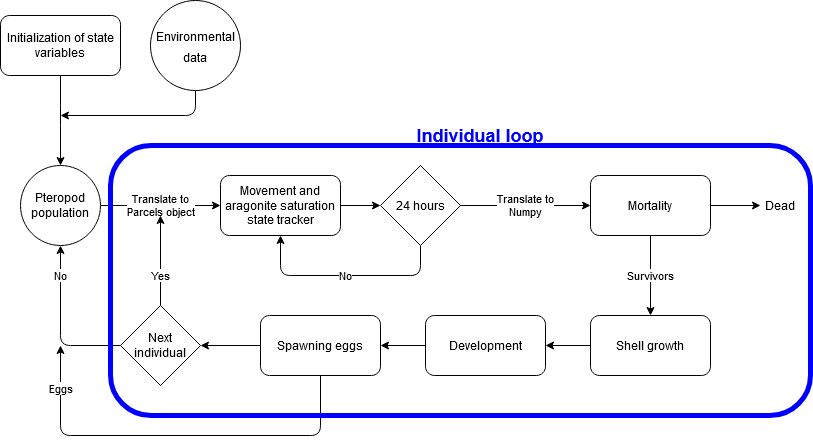
\includegraphics[width=\textwidth]{images/Flow_chart_simple_horizontal.png}
       
    
    \caption{Pteropod individual-based model overview. The blue border shows the processes executed by each simulated pteropod on each one-day time step. }
    \label{fig:flow_chart}
\end{figure*}


% \subsection{Design concepts}\label{sec:design_concepts}
 
% \subsection{Design concepts}\label{sec:design_concepts}
% In this section, we attempt to place our IBM within the eleven concepts identified to capture important characteristics of IBMs \citep{Grimm2010UpdateODD}. Out of the eleven concepts identified in the ODD protocol, our pteropod IBM does not implement objectives (measures used to evaluate decision alternatives), learning (changes in behavior over time), prediction (process by which individuals predict future conditions), interactions (interactions between individuals), or collectives (aggregations of individuals).

\subsection{Design concepts}\label{sec:design_concepts}

% \subsubsection{Basic Principles}\label{sec:basic_principles}
\textit{Basic principles}.  We address the challenges that marine ecosystems face due to climate change. Apart from the global rise in temperature, the global ocean are becoming more acidic due to the marine uptake of anthropogenic CO$_2$ emissions. The rate of ocean acidification, as well as the shoaling of undersaturated waters in productive regions of the world may soon exceed the rate by which populations of marine calcifiers are able to adapt to the new conditions. Thus, this model relates the developmental timings of key traits/organs and behaviours to the size of the pteropods, and the $\Omega_{arag}$ they experience using parameterised responses of pteropods to acidification. This implementations allows the model to be calibrated to a specific region and potentially be extended to include dependencies on other stressors (e.g. deoxygenation).


% Despite the observed widespread dissolution of pteropods in productive regions \citep[CalCS; ][]{Bednarsek2015VerticalDistribution}, a clear picture of the effects of acidification on pteropod populations remains blurry \citep{Doo2020Attribution}. Thus, in this model we relate we base our model on parameterised responses of pteropods to acidification, which allows us to explore the population level response as the sum of the individual responses over time and space.



% Thus, many studies have focused on the individual response of marine calcifiers to projected increases in ocean acidification, and characterize the population level response by extrapolation. However, studies on a population level have not been able to find significant changes caused by ongoing climate change and ocean acidification. As population level studies neglect the size and life stage dependent response to stressors, and sublethal effects, a clear picture of the readily observable effects of climate change remains blurry. This model combines the individual and population level studies, by explicitly representing individuals and their sensitivity to acidification throughout their life cycle, and combining the collective response into a population level response and sensitivity

\textit{Emergence}. Pteropod population size structure, and developmental timings over several generations emerge from their size dependent sensitivity to acidification, repair rates, and the occurrence of undersaturated conditions in relation to their life cycle. As susceptible life stages may co-occur with more corrosive conditions, continuous exposure to corrosive conditions may result in developmental delays that ultimately shift the peak of pteropod abundances and population demographics in future generations. %(\textbf{Need to check this in the results, but this is what I expect to see})

% The key outcome of our IBM, is the dependence of the response of pteropod populations to changes in ocean chemistry on the life stage composition of the population, as well as the occurrence timing of undersaturated conditions. This outcome emerges from the  the size dependent sensitivity to acidification and repair rate, and the two generation life cycle of temperate shelled pteropods where susceptible life stages may co-occur with more corrosive conditions. Additionally, as the development of key traits/organs is dependent on the age and size of the simulated pteropods, the continuous exposure to corrosive conditions may result in developmental delays that ultimately shift the peak of pteropod abundances in future generations. (\textbf{Need to check this in the results, but this is what I expect to see})


\textit{Adaptation}. Pteropods that have developed parapodia adapt their maximum DVM depth during their descent. Pteropods descend in the water column until they reach a maximum depth, which depends on their current size and the maximum depth at the current location. However, if the pteropods reach the upper boundary of the aphotic zone, prior to reaching their maximum DVM depth they will stop descending. This behavior is modeled as indirect objective seeking, i.e. individuals follow rules that have been observed in nature \citep{Grimm2010UpdateODD,Grimm2020SecondUpdateODD}. 
%This rule  takes into account the control of light and phytoplankton biomass on the amplitude of DVM, where for instance in the CalCS, elevated phytoplankton concentrations have been linked to increased light attenuation \citep{Aksnesa2009ShoalingEuphotic}, and decreased in the amplitude of the vertical migration of zooplankton \citep{Ohman2016DVMLight}.

% The pteropod IBM includes a single adaptive behavioral trait. Pteropods have a size-dependent maximum depth, which they aim to reach during their downward migration. However, pteropods can stop their descent at shallower depths if they reach the aphotic zone. This behavior is modeled as indirect objective seeking, i.e. individuals follow rules that have been observed in nature \citep{Grimm2010UpdateODD,Grimm2020SecondUpdateODD}. This rule  takes into account the control of light and phytoplankton biomass on the amplitude of DVM, where for instance in the CalCS, elevated phytoplankton concentrations have been linked to increased light attenuation \citep{Aksnesa2009ShoalingEuphotic}, and decreased in the amplitude of the vertical migration of zooplankton \citep{Ohman2016DVMLight}.
% a depth with a total autotroph production of $0.0\, \frac{mmol C}{m^3s}$.   light availability is low enough. specifically, on each time step during the \textit{DVM and $\Omega_{arag}$ tracker} function each pteropod use a proxy for light availability (total autotroph production in $\frac{mmol C}{m^3s}$) to determine whether 

\textit{Sensing}. Pteropods in our model are assumed to sense their current depth, the light availability, and the time at which the sun sets and rises in each day and location. Our modeled pteropods aim to reach a maximum depth during their downward descent, and upon reaching this depth the descent stops. The pteropods are assumed to simply know the sunrise and sunset time at their current location.
%, where the onset of the downward  and upward migrations occur $21 \pm 20$ minutes before sunrise and $17 \pm 23$ minutes after sunset, respectively \citep{Bianchi2015GlobalDVM}.



\textit{Stochasticity}. Some of processes in our IBM lack the representation of the mechanisms in detail and stochasticity is used instead. Such simplified processes are thus made variable without having to model the cause of the variability  \citep{Grimm2010UpdateODD,Grimm2020SecondUpdateODD}. Specifically, the mechanism by which pteropods sense the sunrise and sunset time at each location is not modeled. Instead we draw a pseudo-random number from a normal distribution with the mean and standard deviation provided for the global DVM patterns \citep{Bianchi2015GlobalDVM}, i.e. $17 \pm 23$ minutes after sunset for the upward migration and  $21 \pm 20$ minutes before sunrise for the downward migration. Another stochastic process in our model is the mortality where an individual dies if a random number between zero and one is greater than its survival probability.


\textit{Observations}. Observations from our IBM include the the abundance of pteropods, population demographics and size structure over time and space, and individual level observations such as the shell size as a function of the experienced $\Omega_{arag}$, age, and generation.


% As the main purpose of this study is to quantify sublethal effects of changing ocean chemistry on populations of shelled pteropods, we collect for each simulated day we collect information on the ID, generation, age, size, and $\Omega_{arag}$ of all simulated pteropods, and determine the distribution of the shell size and $\Omega_{arag}$ across different ages in the spring and overwintering generations. Additionally, for each generation we separate between pteropods that on average experienced low (below 25th percentile) and high (above 75th percentile) $\Omega_{arag}$ throughout their lifetime to contrast the effects of changing ocean chemistry on the size at different ages in the pteropod population. Finally, we extract bulk measures such as the abundance of pteropods to measure whether peaks in abundance coincide with empirical published data \citep[e.g. in ][]{Bednarsek2012PteropodDistribution}.



\subsection{Initialization}\label{sec:initialization}

The initialization should specifically aim to eliminate effects of initial conditions by running the model long enough such that initial conditions have a minimal effect on the model's outcome \citep{Grimm2020SecondUpdateODD}, and thus it is used to define a starting population structure for simulation experiments (section \ref{sec:simulation_experiments}) by mapping the model activity to an observed time series \citep{Grimm2006ODD,Auchincloss2015Healthresearch}. To this end, we ran the IBM for $30'000$ time steps, i.e. around 82 simulation years, starting with a population of $15'000$ eggs of the spring generation, and the processes listed in section \ref{sec:process_overview}, except the \textit{Movement and $\Omega_{arag}$ tracker} function. By excluding this process, the exposure to acidification is turned off, shell growth is not impaired by shell dissolution, and thus simulated pteropods develop without the influence of environmental stressors. The state variables of the initial $15'000$ eggs are as follows: The IDs are set to a number between zero and $14'999$, parent IDs and parent size to $-1$, generation, age and spawning events to zero, ERR to a random number between zero and one, size to $0.15\, mm$ \citep{Wang2017Lifecycle}, and the accumulated damage to $0 \, mg CaCO_3$. The remaining state variables ($\Omega_{arag}$, date, and location) are not initialized at this point, since these state variables are only changed during the execution of the \textit{DVM and $\Omega_{arag}$ tracker} function.


% Next, we parameterise the size of the simulated pteropods as a function of time based on the three-year cohort length-frequency analysis of \textit{L. helicina} spring and overwintering generations in the temperate North Pacific \citep{Wang2017Lifecycle}. The size function describes the (shell) size of pteropods as a function of time using measured length-frequency observations and a variation of the \textit{von Bertalanffy growth function} \citep[VBGF; ][]{Bertalanffy1938}, which considers seasonal changes ($S$) in pteropod growth rates within one year \citep[][]{Wang2017Lifecycle}. The formula used is as follows \citep{Somers1988,GarciaBerthou2012Growth,pauly2013ELEFAN}:
% \begin{eqnarray}
% L(t) & = & L_{\infty} \cdot (1 - e^{-K(t-t_0) - S(t) + S(t_0)}), \\
% S(t) & = & \frac{CK}{\omega} \cdot sin(\omega (t-t_s)), \\
% \omega & = & \frac{2\pi}{T}, \\
% t_s + 0.5\, yr & = & WP,
% \end{eqnarray}
% \noindent
% where $L(t)$ is the size in $mm$ at age $t$ (in years). $t_0$ ($yr$) is the age at which the pteropods have $L=0.0\, mm$, and $t_s$ ($yr$) marks the time of where sinusoidal growth oscillations begin with respect to $t_0$.
% $L_{\infty}$ (in $mm$) denotes the maximum size of the pteropods, $K$ (in $yr^{-1}$) is the rate at which $L_{\infty}$ is approached, $C$ is a unitless factor between zero and one that expresses the amplitude of growth oscillations, $T$ ($yr$) is the period of the oscillation, and $WP$ or winter point ($yr$) indicates the period of the year when growth is minimal. For the spring (overwintering) generation we use the values $WP=0.1\, (0.9)\, yr$, $T=1\, yr$ and $C=0.4\,(1.0)$ as presented in \citet{Wang2017Lifecycle}. The values for $K=5.07\, (4.4)\,yr^{-1}$ and $L_{\infty} = 4.53\,(5.31)\, mm$ are averaged from values reported in \cite{Wang2017Lifecycle} for the spring (overwintering) generations. The length functions for the spring and overwintering generations are shown in figure Fig. \ref{fig:optimal_growth}.

% After the initialization of the pteropod population with $15'000$ eggs, and the calculation of the length function used in the \textit{Shell growth} function, we run the IBM with the \textit{Mortality}, \textit{Shell growth}, \textit{Development}, and \textit{Spawning eggs} functions for $30'000$ time steps, which roughly corresponds to 82 simulation years with spring and overwintering generations. In order to find a pteropod population composition to start the IBM simulation on the 1st January, we calculate an optimal mapping between the abundance of pteropods during the last $10'000$ time steps in chunks of 365 days and the daily abundance data of pteropods interpolated from monthly average and seasonally corrected abundance data found in the temperate region (i.e. between $30\degree$ and $60\degree$ latitude in both hemispheres) reported in the MARine Ecosystem biomass DATa (MAREDAT) initiative \citep{Bednarsek2012PteropodDistribution}. The optimal match was calculated using the Dynamic Time Warping \citep[DTW; ][]{Gupta1996DTW} as implemented in the dtw v1.4.0 python package \citep{giorgino2009computing} with the Manhattan distance. DTW associates each daily abundance in the simulation to a point in the MAREDAT abundance data with the most similar magnitude, while maintaining the sequence of the observations within each data set \citep{Gupta1996DTW}.










% This parameterization does not include an explicit food or temperature limitation, and  found a small correlation between daily growth rates and temperature and phytoplankton biomass \citep{Wang2017Lifecycle}. However, recent work has shown that pteropods can continue growing and overcome periods of food scarcity by using their stored lipids \citep{Maas2020Lipids}.






% The pteropods in our IBM have a longevity of roughly six months as described for the temperate \textit{L. retroversa} individuals under laboratory conditions \citep{Thabet2015Lifestages}. The six month longevity under laboratory conditions has also been observed in the field on the population level for \textit{L. helicina} between spring and summer in the temperate North Pacific \citep{Wang2017Lifecycle}. The development of shelled pteropods under laboratory conditions is comparable to field conditions between spring and summer, where phytoplankton spring blooms and summer production allow the development from egg to reproductive adult within six months \citep{Wang2017Lifecycle}. However, the development of pteropods is linked to their size and thus growth rate. Between autumn and spring, the duration of the larvae stage is extended as a result of overwintering, where pteropod larvae undergo minimal to low growth \citep{Wang2017Lifecycle}, and metamorphose to the juvenile stage in spring \citep{Hunt2008TopPredators}. This delay in growth and development extends the longevity of shelled pteropods to roughly eleven months \citep{Wang2017Lifecycle}. Thus, in addition to the distinction of four stages, we approximate the growth rates of pteropods as a function of time. We use the length-frequency analysis by \cite{Wang2017Lifecycle}  of the three-year cohort analysis of the \textit{L. helicina} populations in the temperate North Pacific to parameterize the growth rates of our pteropods. This parameterization does not include an explicit food or temperature limitation, and  found a small correlation between daily growth rates and temperature and phytoplankton biomass \citep{Wang2017Lifecycle}. However, recent work has shown that pteropods can continue growing and overcome periods of food scarcity by using their stored lipids \citep{Maas2020Lipids}. 

% The growth function assumes two generations per year, a spring generation, and an overwintering generation \citep{Wang2017Lifecycle}. The spring and overwintering generations have a longevity of roughly six months, and eleven months, respectively \citep{Wang2017Lifecycle}. The overwintering generation is characterized by a period of minimal or stagnant growth between November and January \citep{Wang2017Lifecycle}. The growth function describes the length or shell length ($L$) of pteropods as a function of time using measured length-frequency observations and a variation of the \textit{von Bertalanffy growth function} \citep[VBGF; ][]{Bertalanffy1938}, which considers seasonal changes ($S$) in growth rates \citep[Fig. \ref{fig:optimal_growth};][]{Wang2017Lifecycle}. The formula used is as follows \citep{Somers1988,Wang2017Lifecycle}:
% \begin{eqnarray}
% L(t) & = & L_{\infty} \cdot (1 - e^{(K(t-t_0) + S(t) - S(t0))}), \\
% S(t) & = & \frac{CK}{2\pi} \cdot sin(2\pi (t-t_s)), \\
% t_s + 0.5 & = & WP,
% \end{eqnarray}
% \noindent
% where $L(t)$ denotes the length at age $t$, $L_{\infty}$ the maximum length, $K$ how fast $L_{\infty}$ is reached, $C$ the amplitude of growth oscillations, $t_0$ the age at $L=0$, $t_s$ the time between $t=0$ and the onset of oscillations in growth, and $WP$ the fraction of the year where growth is at its slowest. For the spring (overwintering) generation the values of $WP=0.1\,(0.9)$ and $C=0.4\,(1)$ were taken directly from \citep{Wang2017Lifecycle}. The values for $K=5.07\,(4.4)\, s^{-1}$ and $L_{\infty} = 4.53\,(5.31)\, mm$ are average values reported in \cite{Wang2017Lifecycle} for the spring (overwintering) generations. 

% \begin{figure*}[tbh!]
%     \centering
    
%         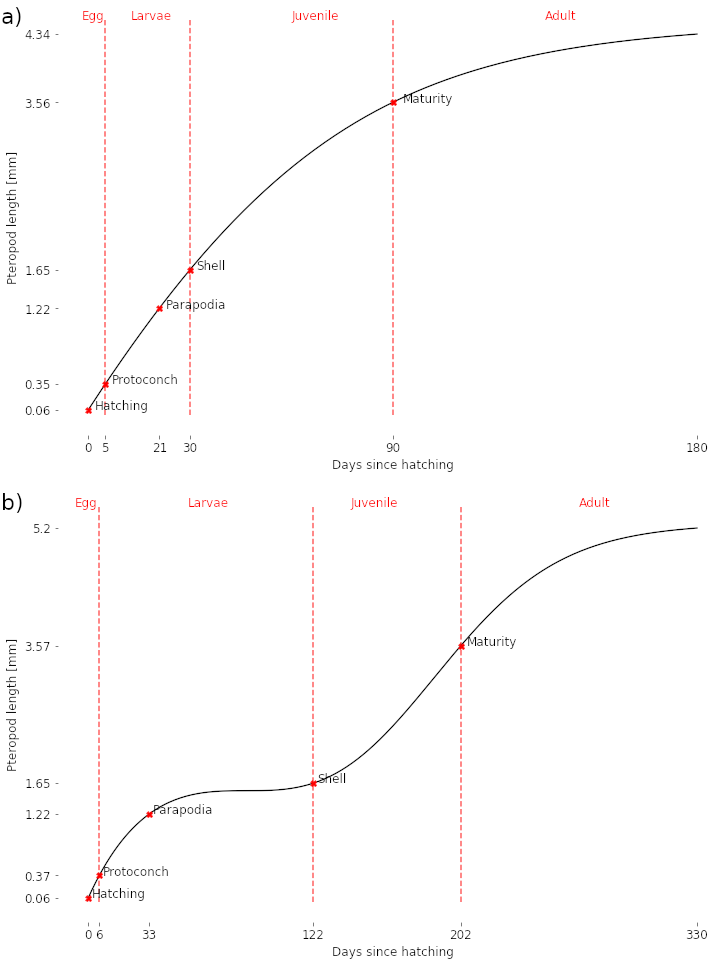
\includegraphics[scale=0.5]{images/Growth_both.png}
       
    
%     \caption{Pteropod length growth (black line) calculated based on the growth rates described in \cite{Wang2017Lifecycle} for the (a) spring generation, and (b) the overwintering generation. The x-axis denotes the days since hatching. The y-axis denotes the length of the pteropod in mm. The red vertical lines separate the growth rate into the life stages, egg, larvae, juvenile, and adult. The red dots mark the hatching at day 0, and the development of key traits such as the protoconch (larval shell), parapodia (wings), shell, and maturity.}
%     \label{fig:optimal_growth}
% \end{figure*}






\subsection{Input Data}\label{sec:input_data}

The input data for the physical-biogeochemical forcing of the IBM needs to be represented by grid cells with the attributes time in days since the start of the simulation, location given as depth ($m$), latitude ($\degree$N) and  longitude ($\degree$E), maximum depth ($m$), land/water index, horizontal and vertical velocities (u, v, and w in $\frac{m}{s}$), the $\Omega_{arag}$, and the total autotroph production in $\frac{mmol}{m^3s}$ (Tab. \ref{tab:state_variables_cells}). In this IBM we used a basin-wide hindcast simulation with daily average output of $\Omega_{arag}$, total phytoplankton productivity, horizontal and vertical velocities of the UCLA-ETH version of the Regional Oceanic Modeling System \citep[ROMS; ][]{shchepetkin2005regional} coupled with the biological elemental cycling model \citep[BEC; ][]{moore2013marine} for the period between 01/01/1979 and 31/12/2016. The hindcast simulation was done using a telescopic grid, which covers the Pacific Ocean basin with a horizontal grid spacing of 60 km that decreases to roughly 4 km towards central California \citep{frischknecht2018origin}. The high resolution at the coast of California properly simulates upwelling conditions along the coastal region, and captures local \citep{frischknecht2018origin}, as well as basin-wide processes \citep{frischknecht2015remote,frischknecht2017local}. With the grid cells of our hindcast simulation, we keep track of the date and location of our pteropods, as well as the $\Omega_{arag}$ that they experience throughout their life.

% The physical-biogeochemical forcing needs to be represented by grid cells with the attributes time in days since the start of the simulation, location given as depth ($m$), latitude ($\degree$N) and  longitude ($\degree$E), maximum depth ($m$), land/water index, horizontal and vertical velocities (u, v, and w in $\frac{m}{s}$), the $\Omega_{arag}$, and the total autotroph production in $\frac{mmol}{m^3s}$ (Tab. \ref{tab:state_variables_cells}).
%, and an unbeaching horizontal velocity in $\frac{m}{s}$ (Tab. \ref{tab:state_variables_cells}).

% The pteropods in our IBM have the attributes date, location, and $\Omega_{arag}$, which are not directly affected by the processes described in section \ref{sec:process_overview}. These three attributes are however changed trough the interaction of pteropods with the environment. In order for our IBM to run, the environment needs to be represented by grid cells with the attributes time in days since the start of the simulation, location given as depth ($m$), latitude ($\degree$N) and  longitude ($\degree$E), maximum depth ($m$), land/water index, horizontal and vertical velocities (u, v, and w in $\frac{m}{s}$), the aragonite saturation state ($\Omega_{arag}$), the total autotroph production ($\frac{mmol}{m^3s}$), and an unbeaching horizontal velocity (Tab. \ref{tab:state_variables_cells}).

% For this study, the environment is taken from a basin-wide hindcast simulation with daily output of $\Omega_{arag}$, total phytoplankton productivity, horizontal and vertical velocities of the UCLA-ETH version of the Regional Oceanic Modeling System \citep[ROMS; ][]{shchepetkin2005regional} coupled with the biological elemental cycling model \citep[BEC; ][]{moore2013marine} for the period between 01/01/1979 and 31/12/2016 starting at $12:05$. The hindcast simulation was done using a telescopic grid, which covers the Pacific Ocean basin with a horizontal grid spacing of 60 km that decreases to roughly 4 km towards central California \citep{frischknecht2018origin}. The refinement in horizontal resolution towards California properly simulates upwelling conditions along the California coastal region, and captures local \citep{frischknecht2018origin}, as well as basin-wide processes \citep{frischknecht2015remote,frischknecht2017local}. With the grid cells of our hindcast simulation, we keep track of the date and location of our pteropods, as well as the environmental conditions they experience throughout their life. %Specifically, the variables of the grid cells (Tab. \ref{tab:state_variables_cells}) are time in days since the start of the simulation, location given as depth ($m$), latitude ($\degree$N) and  longitude ($\degree$E), maximum depth ($m$), land/water index, horizontal and vertical velocities (u, v, and w in $\frac{m}{s}$), the aragonite saturation state ($\Omega_{arag}$), the total autotroph production ($\frac{mmol}{m^3s}$), and an unbeaching horizontal velocity. 


\begin{table*}[h!]
    
    \caption{Description of the variables used to describe the grid cells.}
    \label{tab:state_variables_cells}
    \scriptsize
    \centering
    \begin{tabulary}{\textwidth}{LLL}
    
        \hline
        \textbf{Variable name}                & \textbf{Variable type and units}                       & \textbf{Meaning}                                             \\ \hline
        Time                                   & Static integer in days since start of simulation                           & Identifies the time that has passed since 01/01/1979                          \\ \hline
        Location                            &  Static real numbers for the depth in $m$, the latitude in $\degree$N, and longitude in $\degree$E                           & Links the location of the model to the location in the Pacific Ocean                     \\ \hline
        Maximum depth                      & Static real number in $m$                         & Describes the depth at each grid cell         \\ \hline
        Land/water index                                 & Static integer without units                    & Describes whether a grid cell corresponds to an ocean (1) or land (0) cell                       \\ \hline
        Horizontal and vertical velocities                           & Static real number in $\frac{m}{d}$                       & Describes the horizontal (u and v) and vertical (w) velocities at the edges of each grid cell    \\ \hline
        Aragonite saturation state           & Static real number without units  & Product of concentrations of dissolved calcium and carbonate ions in seawater divided by their product at equilibrium  \\ \hline
        Total autotroph production    & Static real number in $\frac{mmol}{m^3s}$ & Depicts the averaged sum of the production rate of all autotrophs in a given grid cell \\ \hline
        %Unbeaching velocity & Static Real number in $\frac{m}{s}$   & Artificial current that pushes pteropods back to the ocean in case of beaching \citep{Delandmeter2019Unbeaching} \\ \hline
    \end{tabulary}
\end{table*}

% In addition to the representation of the environment, we also require the initial location of our pteropods at the beginning of the simulation. To this end, we input random positions for the simulated pteropod, i.e. we select a random depth, latitude and longitude, which is within a range of latitudes and longitudes of interest. For this project we chose the range between $30-60\degree N$ and $220-245\degree E$, and the depth was set to a fixed depth of $5.0\, m$. Next, we run the model for one year, were the pteropods only execute the \textit{Movement and $\Omega_{arag}$ tracker}. This process results in a list of depths, latitudes, and longitudes to initialize the location attribute for the simulated pteropods around the regions of interest.




% • Whether the model uses any input data to represent variables that change over time or events that occur during a simulation.
% • The input data: what it represents, its units, and its source.
% • Any nontrivial methods used to collect or prepare the input.
% • If input is from another model, how that model was used to generate the input.


\subsection{Submodels}\label{sec:submodels}
All model parameters used for implementing the IBM are summarized in Tab. \ref{tab:parameters}. Their source, function and values are described in the sections below. All submodels use the size of the pteropods for their execution. Thus in contrast to the execution sequence of the submodels (section \ref{sec:process_overview}), we first describe the \textit{Shell growth} function, and build upon the assumption and parameterisations used in this function to describe the \textit{Development}, \textit{Spawning}, \textit{Mortality}, and \textit{Movement and $\Omega_{arag}$ tracker} functions.

\subsubsection{Shell growth}
Each one-day time step, this function calculates the shell growth in four steps for each pteropod (Fig. \ref{fig:shell_growth}). First, we calculate the shell mass ($M_{shell}$) in $mg$ CaCO$_3$. Second, we calculate the shell dissolution as a function of $M_{shell}$ and the $\Omega_{arag}$ that pteropods experienced. Third, we calculate the amount of CaCO$_3$ in $mg$ that pteropods can produce as a function of their current size, and generation. Finally, we calculate the growth or shell repair based on the amount of CaCO$_3$ that can be produced and that was lost due to dissolution.

\begin{figure*}[tbh!]
    \centering
    
        \includegraphics[width=\textwidth]{images/Growth_submodel.png}
       
    
    \caption{Structure of shell growth submodel.}
    \label{fig:shell_growth}
\end{figure*}


\textbf{Step 1:} We estimate the shell mass $M_{shell}$ in $mg$ CaCO$_3$ as a function of the shell length $L$ as presented in \citet{Bednarsek2012Population} and \citet{Bednarsek2014CalcificationDissolution}. The relationship between $M_{shell}$ and $L$ is calculated using an empirical shell length-weight relationship derived from fitting an exponential function to shell length and dry weight ($DW$) measurements of \textit{L. helicina} \citep{Bednarsek2012Population}:

{\scriptsize
\begin{eqnarray}
DW(L) & = & 0.137 \, mg \, dry \, weight \cdot L_{ND}^{1.5005}, \label{eq:dry_weight} \\ 
L_{ND}(L) & = & \frac{L}{1\, mm},
\end{eqnarray}}
\noindent
where $L_{ND}$ is the nondimensionalized version of $L$, L is given in $mm$, and $DW$ in $mg$. Next, we calculate $M_{shell}$ from $DW$. $DW$ is transformed to total carbon content ($TC$ in $mg$) using the average conversion factor $0.25\, \frac{mg TC}{mg DW}$ of dry weight to total carbon of pteropods \citep[][]{Davis1985DWandWW}. The total inorganic carbon ($TIC$) is calculated from $TC$ based on the finding that $27\%$ of the $TC$ correspond to the $TIC$ \citep{Bednarsek2012Population}. $M_{shell}$ is calculate from $TIC$ using the molecular mass ratio of C to CaCO$_3$ ($8.33 \frac{g CaCO_3 \,mol^{-1}}{g TIC\, mol^{-1}}$). This results in the following relationship between $M_{shell}$ and $L$:

{\scriptsize
\begin{eqnarray}
M_{shell}(L) & = & DW(L) \cdot 0.25\frac{mg\, TC}{mg\, dry \, weight} \cdot 0.27\frac{gTIC}{gTC} \cdot 8.33\frac{g\, CaCO_3 \,mol^{-1}}{g\, TIC\, mol^{-1}}. \label{eq:mass_shell}
\end{eqnarray}} 

\textbf{Step 2:} The damage to the shell as a function of the $\Omega_{arag}$ ($Loss_{CaCO_3}$ in $mg$ CaCO$_3$ $d^{-1}$) is calculated based on the empirical fit of a two-parameter exponential function to measurements of the percentage  pteropod shell loss per day ($\nu$ in $\%$ shell loss $d^{-1}$) as a function of $\Omega_{arag}$ in incubation experiments of \textit{L. helicina} \citep{Bednarsek2014CalcificationDissolution}:

{\scriptsize
\begin{eqnarray}
\nu(\Omega_{arag}) & = & 65.76\% \, d^{-1} \cdot e^{-4.7606 \cdot \Omega{arag}}.
\end{eqnarray}}
The $Loss_{CaCO_3}$ is then calculated by multiplying $M_{shell}$ by $\nu$:
{\scriptsize
\begin{eqnarray}
Loss_{CaCO_3}(L,\Omega_{arag}) & = & M_{shell}(L) \cdot \nu(\Omega_{arag}) .
\end{eqnarray}}

\textbf{Step 3:} The amount of CaCO$_3$ that pteropods can produce ($Gain_{CaCO_3}$ in $mg$ CaCO$_3$ $d^{-1}$) is calculated as a function of their current size, their age, generation, and the three-year cohort length-frequency analysis of \textit{L. helicina} spring and overwintering generations in the temperate North Pacific \citep[Fig. \ref{fig:optimal_growth}; ][]{Wang2017Lifecycle}. The latter uses a variation of the \textit{von Bertalanffy growth function} \citep[VBGF; ][]{Bertalanffy1938}, which considers seasonal changes ($S$) in pteropod growth rates within one year \citep[][]{Wang2017Lifecycle}, and is formulated as follows \citep{Somers1988,GarciaBerthou2012Growth,pauly2013ELEFAN}:

{\scriptsize
\begin{eqnarray}
L(t) & = & L_{\infty} \cdot (1 - e^{-K(t-t_0) - S(t) + S(t_0)}),  \label{eq:shell_size}\\
S(t) & = & \frac{CK}{\omega} \cdot sin(\omega (t-t_s)), \\
\omega & = & \frac{2\pi}{T}, \\
t_s + 0.5\, yr & = & WP,
\end{eqnarray}}
\noindent
where $L(t)$ is the size in $mm$ at age $t$ (in years). $t_0$ ($yr$) is the age at which the pteropods have $L=0.0\, mm$, and $t_s$ ($yr$) marks the time sinusoidal growth oscillations begin with respect to $t_0$. $L_{\infty}$ (in $mm$) denotes the maximum size of the pteropods, $K$ (in $yr^{-1}$) is the rate at which $L_{\infty}$ is approached, $C$ is a unitless factor between zero and one that expresses the amplitude of growth oscillations, $T$ ($yr$) is the period of the oscillation, and $WP$ or winter point ($yr$) indicates the fraction of the year when minimal growth begins. For the spring (overwintering) generation (Fig. \ref{fig:optimal_growth}) we use the values $WP=0.1\, (0.9)\, yr$, $T=1\, (1)\, yr$ and $C=0.4\,(1.0)$ as presented in \citet{Wang2017Lifecycle}. The values for $K=5.07\, (4.4)\,yr^{-1}$ and $L_{\infty} = 4.53\,(5.31)\, mm$ are averaged from values reported in \cite{Wang2017Lifecycle} for the spring (overwintering) generations. The total life span of the spring (overwintering) generation is 180 (330) days \citep{Wang2017Lifecycle}. This parameterisation does not include an explicit food or temperature limitation \citep{Wang2017Lifecycle}. However, periods of rapid growth coincide with spring blooms and high summer productivity \citep{Wang2017Lifecycle,Maas2020Lipids}. Alternatively, periods of minimal growth are associated with lower chlorophyll-a concentrations and the onset of winter \citep{Wang2017Lifecycle,Maas2020Lipids}.


First, we calculate the gradient of $L(t)$ to find the shell length increase ($dL$) in a one-day time step for the age and generation of a pteropod. $Gain_{CaCO_3}$ is then calculated as the amount of CaCO$_3$ that the pteropod would produce if it increases its shell size by $dL$. Explicitly, we calculate the shell mass as a function of the sum of the current shell size and $dL$ (eq. \ref{eq:mass_shell}), and subtract the shell mass calculated in step 1:

{\scriptsize
\begin{eqnarray}
Gain_{CaCO_3}(L,dL) & = & M_{shell}(L+dL) - M_{shell}(L).
\end{eqnarray}}

\textbf{Step 4:} We calculate the net amount of CaCO$_3$ that remains after dissolution and calcification:

{\scriptsize
\begin{eqnarray}
Net_{CaCO_3} & = & Gain_{CaCO_3} - Loss_{CaCO_3}.
\end{eqnarray}}
\noindent
If $Net_{CaCO_3}$ is negative or zero ($Gain_{CaCO_3} \leq Loss_{CaCO_3}$), then neither growth nor shell repair occurs, and the accumulated damage state variable is increased by the absolute value of $Net_{CaCO_3}$. If $Net_{CaCO_3}$ is positive ($Gain_{CaCO_3} > Loss_{CaCO_3}$) and the accumulated damage is zero, then $Net_{CaCO_3}$ is added to  $M_{shell}(L)$ and the increase in size is calculated as the inverse of equations (\ref{eq:mass_shell}) and (\ref{eq:dry_weight}). If $Net_{CaCO_3}$ is positive, and the accumulated damage is larger or equal to  $Net_{CaCO_3}$, then the accumulated damage is repaired, i.e. it is reduced by the absolute value of $Net_{CaCO_3}$ without increasing the size state variable. Finally, if $Net_{CaCO_3}$ is positive, and the accumulated damage is smaller than $Net_{CaCO_3}$, then the accumulated damage is repaired and the remaining amount of CaCO$_3$ is added to  $M_{shell}(L)$ and the increase in size is calculated as the inverse of equations (\ref{eq:mass_shell}) and (\ref{eq:dry_weight}).



\subsubsection{Development}
Each one-day time step, this function determines the life stage that a pteropod has reached depending on their size. The life stage is not a state variable as it can be derived from the size state variable \citep{Grimm2010UpdateODD}. However, we introduce life stages as it facilitates the analysis of the model output by binning individuals that share physiological and behavioral characteristics (i.e. protoconch, parapodia, juvenile/adult shell, maturity) into categories. To this end, we link the development of these characteristics to the shell size using the developmental timings of these characteristics in culturing experiments \citep{Howes2014Lab,Thabet2015Lifestages}, and the shell size parameterisation ($L(t)$, eq. (\ref{eq:shell_size})) for the spring generation \citep{Wang2017Lifecycle}. We chose the spring generation, since both culturing experiments and the spring generation have the same life span of six months \citep{Howes2014Lab,Thabet2015Lifestages,Wang2017Lifecycle}. 

The life stages are based on the ten-stage life cycle of \textit{L. retroversa} \citep{Howes2014Lab,Thabet2015Lifestages}. We simplify the ten-stage life cycle into four life-stage tracer (Fig. \ref{fig:optimal_growth}):  the eggs (containing the 2-, 4-, 8-, 16-cell, blastula, gastrula, and trochophore stages), larvae (containing the veliger stage), juveniles (containing the non-reproductive juveniles), and reproductive adults. These four life stages are coded as zero, one, two, and three for eggs, larvae, juveniles, and adults, respectively. The transition from egg to larvae is based on the formation of the protoconch after six days of development \citep{Thabet2015Lifestages} which corresponds to a size of $0.56 \, mm$. During the larvae stage, pteropods develop parapodia after 21 days of development \citep{Thabet2015Lifestages}. The transition from larvae to juvenile is based on the formation of the juvenile shell after 30 days of development \citep{Thabet2015Lifestages} which corresponds to a size of $1.79 \, mm$. The transition from juvenile to adult is based on the development of female gonads after 90 days of development \citep{Thabet2015Lifestages} which corresponds to a size of $3.70 \, mm$. These size thresholds are then used to determine the life stages of both the spring and overwintering generations. After determining the life stage, the age of the pteropods is increased by one day.

\begin{figure*}[tbh!]
    \centering
    
        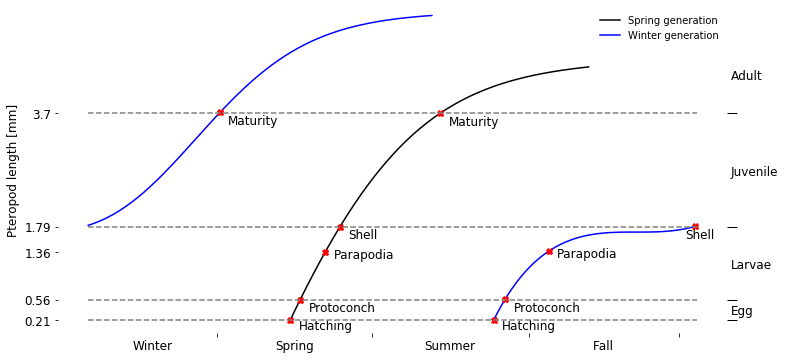
\includegraphics[width=\textwidth]{images/Growth_functions.png}
       
    
    \caption{Size of pteropods parameterised as a function of time for the spring (black) and overwintering (blue) generations \citep{Wang2017Lifecycle}. Annotated in red are the sizes at which pteropods hatch ($0.21 \, mm$), develop a protoconch (larval shell; $0.56 \, mm$), parapodia (wings; $1.36 \, mm$), juvenile/adult shell ($1.79 \, mm$) or reach maturity ($3.70 \, mm$) based on the comparison between culturing experiments \citep{Howes2014Lab,Thabet2015Lifestages}, and the parameterisation for the spring generation. The life stages (egg, larvae, juvenile, and adult) are shown on the right.}
    \label{fig:optimal_growth}
\end{figure*}

\subsubsection{Spawning}
Each one-day time step, this function determines whether a pteropod has reached maturity and is ready to spawn eggs. Eggs are released by adults as buoyant free-floating masses at the water surface \citep{Lalli1978Reproduction,Paranjape1968egg,Schalk1990SeasonalSpatial,Gannefors2005Overwintering,Comeau2010Predation,Manno2016EggsAcidification}. Synchronized widespread spawning takes place in spring and autumn \citep{lalli1989pelagic,Thabet2015Lifestages,Wang2017Lifecycle}. The number of eggs released per reproductive pteropod adults has a high variability, which is likely linked to the environmental conditions that pteropods experience \citep{Manno2016EggsAcidification}. For instance, the number of eggs released range between $524$ and $10'051$ (mean $5'936$) per \textit{Limacina helicina} female in the arctic \citep{Lalli1978Reproduction}, and between $465$ and $708$ eggs (mean $565$) in the temperate region \citep{Paranjape1968egg}. Additionally, the number of eggs released by adults depends on the pteropod species, where the temperate to subpolar \textit{L. retroversa} females released  between $83$ and $650$ (mean $260$) eggs in a $20$ day period \citep{Lalli1978Reproduction}.

This function models the pause between spawning events using an Egg Release Readiness (ERR) index \citep[similar to the Clutch Readiness Fraction presented in ][]{Miller1998CalanusIBM}. The ERR index is set to a random number between zero and one when the eggs are released (section \ref{sec:initialization}), it increases by $\frac{1}{20}$ each day if the pteropod has reached the adult life stage, and upon reaching $ERR \geq 1.0$ the eggs are released. Thus, this function first searches for all adult pteropods. The ERR values of those with an $ERR \geq 1.0$ (i.e. those that spawned eggs in the previous time step), are reset to zero. The ERR values of those with $ERR < 1.0$, are increased by $\frac{1}{20}$. Second, as we are interested in simulating the synchronized widespread spawning events in spring and autumn \citep{lalli1989pelagic,Thabet2015Lifestages,Wang2017Lifecycle} and neglect continuous low level spawning throughout the year \citep{Wang2017Lifecycle,Thabet2015Lifestages}, only adults of the youngest generation spawn eggs in our model, i.e. if adults of the overwintering and spring generation are present, only the adults of the latter will spawn eggs. Third, this function selects adult pteropods of the youngest generation with an $ERR \geq 1.0$. Each of the selected adults spawn 500 eggs. In our model we use a conservative estimate of $500$ eggs per spawning event, which is within the ranges reported for \textit{L. retroversa} and \textit{L. helicina} in the arctic and temperate regions. After the spawning events, the state variable spawning events of the selected adults is increased by one.

The state variables of the eggs are initialized as follows: The IDs are set to unique integer based on the largest ID used before the spawning events and the number of eggs released, parent IDs and parent size are set to the IDs and sizes of the respective pteropods that produced the eggs, generation is set to the generation of the parent plus one, age and spawning events to zero, ERR to a random number between zero and one, size to $0.15\, mm$ \citep{Wang2017Lifecycle} and the accumulated damage to $0 \, mg CaCO_3$. The remaining state variables ($\Omega_{arag}$, date, and location) are initialized in the \textit{Movement and $\Omega_{arag}$ tracker} function.



% In our model we use a conservative estimate of $600$ eggs per spawning event \citep{Paranjape1968egg}, which is within the ranges reported for \textit{L. retroversa} and \textit{L. helicina} in the arctic and temperate regions. During spawning a pause of roughly 20 days has been observed between separate spawning events \citep{Paranjape1968egg}.




% After updating the ERR values of the adult pteropods, the function selects the pteropods with an $ERR \geq 1.0$. Each of the selected adults spawn 500 eggs. Eggs are released by adults as buoyant free-floating masses at the water surface \citep{Lalli1978Reproduction,Paranjape1968egg,Schalk1990SeasonalSpatial,Gannefors2005Overwintering,Comeau2010Predation,Manno2016EggsAcidification}.




% During spawning a pause of roughly 20 days has been observed between separate spawning events \citep{Paranjape1968egg}. We model this pause using an Egg Release Readiness (ERR) index \citep[similar to the Clutch Readiness Fraction presented in ][]{Miller1998CalanusIBM}. The ERR index is set to a random number between zero and one when the eggs are released (section \ref{sec:initialization}), it increases by $\frac{1}{20}$ each day if the pteropod has reached the adult life stage, and upon reaching $ERR \geq 1.0$ the eggs are released, and ERR is set to zero. Thus in this function 


% Eggs are released by adults as buoyant free-floating masses at the water surface \citep{Lalli1978Reproduction,Paranjape1968egg,Schalk1990SeasonalSpatial,Gannefors2005Overwintering,Comeau2010Predation,Manno2016EggsAcidification}. There is evidence for continuous low level spawning  throughout the year \citep{Wang2017Lifecycle,Thabet2015Lifestages}, but synchronized widespread spawning takes place in spring and autumn \citep{lalli1989pelagic,Thabet2015Lifestages,Wang2017Lifecycle}. The number of eggs released per reproductive pteropod adults has a high variability, which is likely linked to the environmental conditions that pteropods experience \citep{Manno2016EggsAcidification}. For instance, the number of eggs released range between $524$ and $10'051$ (mean $5'936$) per \textit{Limacina helicina} female in the arctic \citep{Lalli1978Reproduction}, and between $465$ and $708$ eggs (mean $565$) in the temperate region \citep{Paranjape1968egg}. Additionally, the number of eggs released by adults depends on the pteropod species, where the temperate to subpolar \textit{L. retroversa} females released  between $83$ and $650$ (mean $260$) eggs in a $20$ day period \citep{Lalli1978Reproduction}. In our model we use a conservative estimate of $600$ eggs per spawning event \citep{Paranjape1968egg}, which is within the ranges reported for \textit{L. retroversa} and \textit{L. helicina} in the arctic and temperate regions. During spawning a pause of roughly 20 days has been observed between separate spawning events \citep{Paranjape1968egg}. We model this pause using an Egg Release Readiness (ERR) index \citep[similar to the Clutch Readiness Fraction presented in ][]{Miller1998CalanusIBM}. The ERR index is set to a random number between zero and one at maturation, it increases by $\frac{1}{20}$ each day, and upon reaching $ERR \geq 1.0$ the eggs are released, and ERR is set to zero. 



\subsubsection{Mortality}
Information on the mortality rates of pteropods is scarce \citep{Lischka2011WarmingAcidificationJuveniles,Bednarsek2012Population,Bednarsek2016CumulativeEffects}. Thus we modeled the mortality of the pteropods in our model as a stochastic process. Each pteropod has a fixed size- and generation-specific mortality coefficient (henceforth called mortality coefficient). On each one-day time step, a pseudo-random number is drawn from a discrete uniform distribution, and if the pseudo-random number is smaller or equal to the mortality coefficient ($Mort_{coeff}$), the pteropod dies. To this end, we estimate the mortality coefficient based on an exponential decline in the number of individuals over time \citep{Bednarsek2012Population,Bednarsek2016CumulativeEffects}:

{\scriptsize
\begin{eqnarray}
N_{t+1} & = & N_{t}\cdot e^{-\beta \cdot 1\, d},
\end{eqnarray}}
\noindent
where $N_{t}$ is the number of individual at time $t$, $\beta$ is the mortality rate ($d^{-1}$), and $e^{-\beta \cdot t}$ the fraction of individuals that survive into the next time step ($N_{t+1}$). The mortality coefficient was then defined as:
{\scriptsize
\begin{eqnarray}
Mort_{coeff} & = & 1 - e^{-\beta \cdot 1\, d}.
\end{eqnarray}}
\noindent
The mortality rates for each life-stage (egg, larvae, juvenile, adult) were calibrated for the simulation experiments (section \ref{sec:simulation_experiments}), since information on daily mortality rates \citep[$\beta$; ][]{Bednarsek2016CumulativeEffects}  or mortality coefficients \citep{Lischka2011WarmingAcidificationJuveniles} for different life stages is scarce, and reported values show large variability. For instance juvenile \textit{L. helicina} collected in Kongsfjord had a mean mortality coefficient of $12.6\%$ \citep{Lischka2011WarmingAcidificationJuveniles} whereas the mortality coefficient for juvenile \textit{L. helicina} in the Scotia Sea is around $1.0 \%$ \citep{Bednarsek2012Population,Bednarsek2016CumulativeEffects}. Other processes modeled in this function are the mortality due to old age \citep{Wang2017Lifecycle} and after spawning events \citep{Wang2017Lifecycle}. Pteropods of the spring and overwintering generation can live up to 180 days \citep{Howes2014Lab,Thabet2015Lifestages,Wang2017Lifecycle} and 330 days \citep{Wang2017Lifecycle}, respectively. In addition, adult pteropods die if they have had two spawning events. This is based on the observations that pteropods die shortly after spawning events \citep{Dadon1992Reproduction,Gannefors2005Overwintering,Hunt2008TopPredators,Howes2014Lab}, and only a few adults have been observed to spawn eggs twice in a 20 day window \citep{Paranjape1968egg}.





\subsubsection{Movement and $\Omega_{arag}$ tracker}
This function calculates the horizontal and vertical advection of the pteropods, their vertical migration, and keeps track of their exposure to $\Omega_{arag}$. This is done using three subroutines executed in parallel. The first one calculates the horizontal and vertical advection of the pteropods, the second one calculates the vertical migration of pteropods, and the third one samples the $\Omega_{arag}$ at the current location of the pteropods.

In the first subroutine, the advection is calculated using parcels' built-in fourth-order Runge-Kutta integration scheme, which includes the vertical velocity \citep{Delandmeter2019Unbeaching}. The integration uses a time step of one hour to calculate the position of the pteropods between the horizontal and vertical velocities of two daily average outputs taken from the physical-biogeochemical forcing (section \ref{sec:initialization}). However, this advection scheme has been reported to result in beaching of particles \citep{Delandmeter2019Unbeaching}. Thus, as suggested in \cite{Delandmeter2019Unbeaching}, we implemented an artificial current that pushes pteropods back to the ocean if they are advected onto the shore, below the maximum depth, or above the surface.

\textbf{Subroutine 2:} We simulate the DVM for pteropods that develop parapodia at a size of $1.36 \, mm$ (Fig. \ref{fig:optimal_growth}.

\textbf{Subroutine 3:}






This function computes secondary attributes that are derived from the size, date and location state variables of each pteropod. The secondary attributes are used to calculate the vertical movement of the pteropods during the execution of the \textit{Movement and $\Omega_{arag}$ tracker} function, and include the upward and downward swimming speeds, the maximum DVM depth, and the time at which the downward and upward migration starts. 
%With the development of parapodia at a size of $1.22\,mm$ (Fig. \ref{fig:optimal_growth}), pteropods counteract the negatively buoyant aragonite shell \citep{Byrne1984SettlingSpeed,Bergan2017SwimmingSinkingSpeeds} by swimming upwards in the water column \citep{Murphy2016UpwardSwimming}. 
The upward swimming speed ($v_{up}$) of shelled pteropods varies between $13 \, mm \, s^{-1}$ for smaller pteropods and reaches $44\, mm\, s^{-1}$ for the largest ones \citep{Chang2012SwimmingSpeedSize}. We define $44\, mm\, s^{-1}$ as the maximum swimming speed of our pteropods, and approximate the effect of increasing size by multiplying the maximum swimming speed with the current shell length ($L$) to maximum shell length $L_{\infty} = 5.31\, mm$ ratio (section \ref{sec:growthRates}).
Thus, for a pteropod with $L = 1.6\,mm$ we model a swimming speed of roughly $13.3 \, mm \, s^{-1}$, which is within the range provided by \cite{Murphy2016UpwardSwimming} for pteropods with this shell length. Similarly, the sinking speed ($v_{down}$) was modeled using a maximum terminal swimming speed of $18\, mm\, s^{-1}$ \citep{Bergan2017SwimmingSinkingSpeeds} and scaled with the current shell length to maximum shell length $L_{\infty}$ ratio, which takes into account the mass loss on the sinking velocity \citep{Byrne1984SettlingSpeed}. The formulas are thus given as
\begin{eqnarray}
v_{up}(L) & = & 44 \, \frac{mm}{s} \cdot \frac{L}{L_{\infty}},\\
v_{down}(L) & = & 18 \, \frac{mm}{s} \cdot \frac{L}{L_{\infty}}.
\end{eqnarray}


In order to model DVM, also require the sinking depth, as well as the onset of the downward and upward migration. For the DVM depth ($d_{DVM}$ in $m$), we use observations reported for the California Current System, where pteropods are mainly found in waters above $250\, m$ \citep{Bednarsek2015VerticalDistribution}. The DVM depth increases with pteropod size, i.e. smaller pteropods are primarily located at the surface, and the largest ones sink to deeper layers  \citep{Bednarsek2015VerticalDistribution}. Thus, we chose a maximum DVM depth of $250\, m$ and calculate for each pteropod their maximum DVM depth by multiplying the maximum DVM depth with their current shell length to maximum shell length $L_{\infty}$ ratio:
\begin{eqnarray}
d_{DVM}(L) & = & 250\, m \cdot \frac{L}{L_{\infty}}.
\end{eqnarray}
The onset of the downward ($t_{down}$) and upward ($t_{up}$) migration are calculated based on the global DVM patterns of zooplankton, where pteropods start swimming downwards $21\pm 20\, min$ before sunrise, and arrive at the surface from their maximum DVM depth $17\pm 23\, min$ after sunset \cite{Bianchi2015GlobalDVM}. The sunrise and sunset timings are calculated using the astral v2.2 python package \citep{astral2020}. Specifically, for $t_{up}$ we draw a pseudo-random from a normal distribution with $\mu=17\,min$ and $\sigma=23\,min$, and add it from the sunset time ($t_{sunset}$) to obtain the time at which pteropod arrive at the surface $t_{surface}$. Next, as we are interested in the time at which the pteropods start their upward migration, we calculate the time each pteropod would theoretically need to reach the surface from their maximum DVM depth ($d_{DVM}$) with the given upward swimming speed ($v_{up}$), and subtract it from the time at which pteropods reach the surface. For $t_{down}$ we first draw a pseudorandom number from a normal distribution ($\mathcal{N}(\mu,\,\sigma)$) with the mean ($\mu$) and standard deviation ($\sigma$) of $21$ and $20\,min$, and subtract it from the sunrise time of the following day ($t_{sunrise}$). We add one day before calculating $t_{sunrise}$, since the movement of pteropods is calculated for 24 hours starting at $12:05$. Thus the upward migration takes place on the same day around sunset, whereas the downward migration takes place on the next day around sunrise.
\begin{eqnarray}
t_{down} & = & t_{sunrise} - \mathcal{N}(\mu=21\,min,\,\sigma=20\,min), \\
t_{surface} & = & t_{sunset} + \mathcal{N}(\mu=17\,min,\,\sigma=23\,min), \\
t_{up} & = & t_{surface} - \frac{d_{DVM}}{v_{up}}.
\end{eqnarray}




This function computes the advection and DVM of our pteropods using the Lagrangian ocean analysis tool Parcels v2.1.3 \citep{Delandmeter2019Unbeaching}. The advection was calculated using parcels' built-in fourth-order Runge-Kutta integration scheme, which includes the vertical velocity \citep{Delandmeter2019Unbeaching}. The integration uses a time step of one hour to calculate the position of the pteropods between two daily outputs. However, this advection scheme has been reported to result in beaching of particles \citep{Delandmeter2019Unbeaching}. Thus, as suggested in \cite{Delandmeter2019Unbeaching}, we implemented an artificial current that pushes our pteropods back to the ocean if they are advected onto the shore. In addition to the advection and unbeaching velocities, pteropods that reach a size of $1.22\,mm$ (Fig. \ref{fig:optimal_growth}) develop parapodia, and are thus able to perform DVM.

The DVM submodel begins by constraining the maximum DVM depth ($d_{DVM}$) to the maximum water column depth ($d_{max}$) if $d_{DVM}>d_{max}$. Pteropods approach the surface with $v_{up}$ if the current time ($t_{curr}$) is larger or equal to $t_{up}$ and below or equal to $t_{down}$. Upon reaching the surface, pteropods passively drift at the surface. If $t_{current}$ is above $t_{down}$ or below $t_{up}$, pteropods swim downwards with $v_{down}$ towards their DVM depth $d_{DVM}$. Pteropods can stop their descent at a shallower depth, if they reach a region of zero productivity, which we assume to roughly coincide with the start of the aphotic zone. Upon reaching their DVM depth, pteropods try to keep this DVM depth and drift.

During the vertical migration, pteropods sense total autotroph production and the $\Omega_{arag}$ of their surroundings. At each time step, the simulated pteropods sample the $\Omega_{arag}$ at their current location, and add it to the daily running total (cumulative sum) $\Omega_{arag}$. The daily running total $\Omega_{arag}$ is then divided by the number of time steps in the \textit{Movement and $\Omega_{arag}$ tracker} function to calculate the average $\Omega_{arag}$ experienced on each day.









\subsection{Calibration}

\subsection{Simulation experiments}\label{sec:simulation_experiments}

\section{Old version below}



% In addition to the dissolution, pteropods are able to repair their shells \citep{Bednarsek2014CalcificationDissolution}. Thus we also calculate the gain of CaCO$_3$ or calcification (in $mg$ CaCO$_3$) for a pteropod of length $L$ (in $mm$) that is exposed to a aragonite saturation state $\Omega_{arag}$. First, we calculate the rate of calcification ($Q$ in $\frac{\mu mol \, CaCO_3}{g Wet weight h}$) as presented in \citep{Comeau2010RepairRates}. Next, we calculate the wet weight of a pteropod with length $L$ \citep[$WW$ in $g$; ][]{Bednarsek2014CalcificationDissolution}. Finally, we multiply $Q$, $WW$, and the molar mass of CaCO$_3$ ($100.09 \frac{g}{mol}$) to get the gain of CaCO$_3$ in $\mu g$ CaCO$_3$ $h^{-1}$, which we transform to $mg$ CaCO$_3$ $d^{-1}$ and multiply by one day to match the units of the loss term mentioned in above:
% \begin{eqnarray}
% Q & = & 0.57 \cdot ln(\Omega_{arag}) + 0.25, \\
% WW & = & \frac{DW}{0.28 \cdot 1'000}, \\
% gain & = & Q \cdot WW \cdot 100.09 \cdot 1'000 \cdot 24 \cdot 1.
% \end{eqnarray}
% \noindent
% The definition of the loss and gain terms as $mg$ CaCO$_3$ allows us to calculate the net effect of acidification on the shell growth, where after each day we calculate the deviation from the optimal shell growth defined for the spring and overwintering populations if the loss term exceeds the gain term. Additionally, since both calcification and dissolution are calculated as functions of $L$, our model takes the sensitivity of different stages into account, where early life stages are more sensitive to acidification relative to the adults (not shown, \textbf{preparing plot}).
% Thus, using the size or shell length to define the transition between life stages, and the development of traits (e.g. parapodia, shell, maturity), we can simulate the net effect of acidification on the developmental timings of pteropod traits throughout their life, or the deviation from optimal growth.




% \subsubsection{Develop}
% \begin{itemize}
%     \item threshold definitions for traits using length as function of time and developmental timings of lab experiments
%     \item stages
%     \item Combining time since birth and shell size
%     \item ERR index
% \end{itemize}

% \subsubsection{Spawn eggs}
% \begin{itemize}
%     \item difference between generations
%     \item number of eggs
%     \item location of release
%     \item ERR
% \end{itemize}










% \section{Robustness tests of the model}

% IBMs are a widely used tool to infer the impacts and responses of a changing environment on populations or communities on a regional or global scale \citep{DeAngelis2014IBM}. The organism chosen for the IBM can vary between a wide group \citep[e.g. phytoplankton; ][]{Clark2011IBMAdaptations} or a specific species \citep[e.g. Calanus finmarchicus, three-spined stickleback; ][]{Miller1998CalanusIBM,Mintram2018IBM_Stickleback}. Due to the species-specific dependence of pteropod growth rates and longevity to environmental conditions  \citep[e.g. temperature, food availability; ][]{Wang2017Lifecycle}, we focus herein on the group of shelled pteropods instead of individual species. This allows us include broad individual-level processes and behaviours \citep{DeAngelis2014IBM}, such as changes in acidification sensitivity along the life-cycle of the pteropods \citep{Bednarsek2016CumulativeEffects}, their calcification rate with changing shell size \citep{Bednarsek2014CalcificationDissolution}, their exposure to acidification due to DVM with increasing size \citep{Maas2012DVM,Bednarsek2015VerticalDistribution}, as well as changes in their abundance or shell dissolution and size across several generations.


% \section{Coupling to circulation model}
% The grid cells are taken from a basin-wide hindcast simulation with daily output of $\Omega_{arag}$, total phytoplankton productivity, horizontal and vertical velocities of the UCLA-ETH version of the Regional Oceanic Modeling System \citep[ROMS; ][]{shchepetkin2005regional} coupled with the biological elemental cycling model \citep[BEC; ][]{moore2013marine} for the period between 01/01/1979 and 31/12/2016. The hindcast simulation was done using a telescopic grid, which covers the Pacific Ocean basin with a horizontal grid spacing of 60 km that decreases to roughly 4 km towards central California \citep{frischknecht2018origin}. The refinement in horizontal resolution towards California properly simulates upwelling conditions along the California coastal region, and captures local \citep{frischknecht2018origin}, as well as basin-wide processes \citep{frischknecht2015remote,frischknecht2017local}. With the grid cells of our hindcast simulation, we keep track of the time and location of our pteropods, as well as the environmental conditions they experience throughout their life. Specifically, the attributes of the grid cells (Tab. \ref{tab:state_variables_cells}) are time in days since the start of the simulation, location given as depth ($m$), latitude ($\degree$N) and  longitude ($\degree$E), maximum depth ($m$), land/water index, horizontal and vertical velocities (u, v, and w in $\frac{m}{s}$), the aragonite saturation state ($\Omega_{arag}$), the total autotroph production ($\frac{mmol}{m^3s}$), and an unbeaching horizontal velocity. 


% \begin{table}[tbh!]
%     \label{tab:state_variables_cells}
%     \caption{Description of the state variables used to describe the grid cells.}
%     \centering
%     \begin{tabulary}{0.8\textwidth}{LLL}
    
%         \hline
%         \textbf{Variable name}                & \textbf{Variable type and units}                       & \textbf{Meaning}                                             \\ \hline
%         Time                                   & Static integer in days since start of simulation                           & Identifies the time that has passed since 01/01/1979                          \\ \hline
%         Location                            &  Static real numbers for the depth in $m$, the latitude in $\degree$N, and longitude in $\degree$E                           & Links the location of the model to the location in the Pacific Ocean                     \\ \hline
%         Maximum depth                      & Static real number in $m$                         & Describes the depth of each grid cell         \\ \hline
%         Land/water index                                 & Static integer without units                    & Describes whether a grid cell corresponds to an ocean (1) or land (0) cell                       \\ \hline
%         Horizontal and vertical velocities                           & Static real number in $\frac{m}{d}$                       & Describes the horizontal (u and v) and vertical (w) velocities at the edges of each grid cell    \\ \hline
%         Aragonite saturation state           & Static real number without units  & Product of concentrations of dissolved calcium and carbonate ions in seawater divided by their product at equilibrium  \\ \hline
%         Total autotroph production    & Static real number in $\frac{mmol}{m^3s}$ & Depicts the averaged sum of the production rate of all autotrophs in a given grid cell \\ \hline
%         Unbeaching velocity & Static Real number in $\frac{m}{s}$   & Artificial current that pushes pteropods back to the ocean in case of beaching \citep{Delandmeter2019Unbeaching} \\ \hline
%     \end{tabulary}
% \end{table}



% The pteropod IBM is structured in two modules, a population module, and a physical module \citep[similar to ][]{Miller1998CalanusIBM}. The population module simulates a simplified life cycle of shelled pteropods parameterized using compiled published experimental data on temperate pteropod life history, behavioral, physiological and morphological traits. The physical module computes the movement (i.e. advection and DVM) of the pteropods, and keeps track of the environmental conditions that the pteropods experience each day.  We based our model on temperate pteropod species, since the highest biomass of shelled pteropods has been recorded in the temperate region \citep{Bednarsek2012PteropodDistribution}, and compared to polar species, temperate species show a lower dependence of growth and longevity on seasonal changes in environmental factors \citep[e.g. temperature and food availability][]{Bednarsek2012PteropodDistribution,Wang2017Lifecycle,Manno2017ReviewPteropodVulnerability}. The processes that we simulate in the coupled physical-biological model are visualized in figure \ref{fig:model_visualization}, and explained in the following sections.



% Each pteropod is represented as a vector containing $24$ parameters (Tab. \ref{tab:parameters}) used to model the life history, physiological, morphological, and behavioral traits of pteropods, which are explained in the following sections.

\begin{figure*}[tbh!]
    \centering
    
        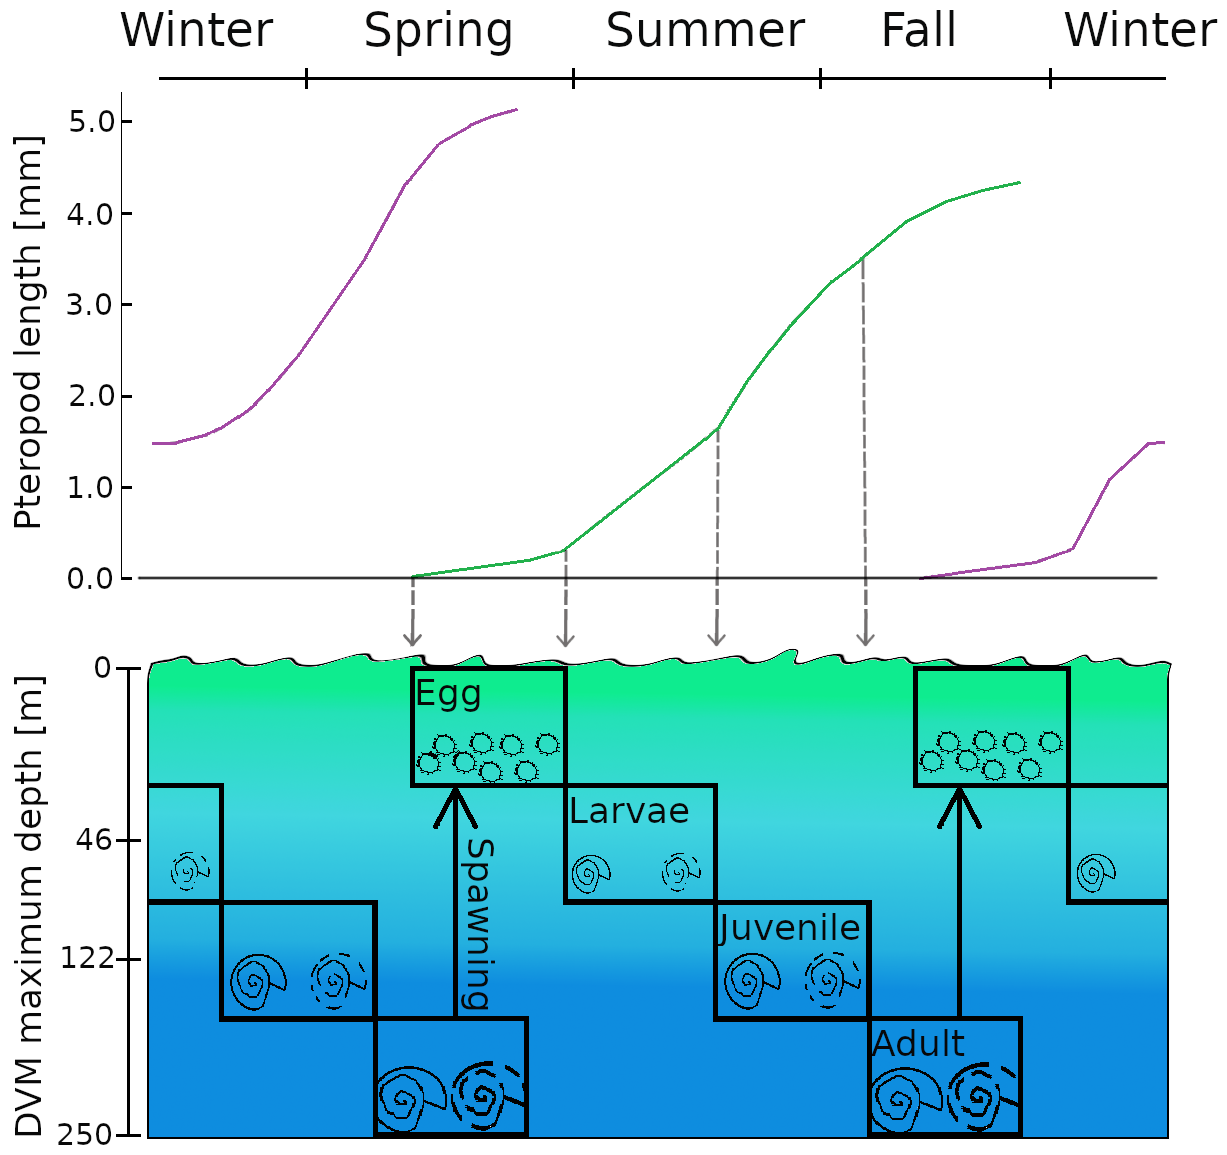
\includegraphics[scale=0.5]{images/Model_sketch_V2_stages.png}
       
    
    \caption{Visualization of the processes included in the pteropod IBM model. At the top is the length of a pteropod in $mm$ as a function of the season normalized to the length of each life stage (grey downward arrows). Below are the four stages (egg, larvae, juvenile, and adult) included in the population module shown by the boxes. The spawning events are marked by the black upward arrows. The maximum depth of diurnal vertical migration (DVM) is shown in the y-axis, where the egg stage remains at the surface, and all other stages perform DVM. Stages affected by dissolution by the shells with gaps.}
    \label{fig:model_visualization}
\end{figure*}


\subsection{Population module}

\subsubsection{Life cycle of pteropods}
We simplify the ten-stage life cycle of shelled pteropods \citep{Howes2014Lab,Thabet2015Lifestages} into four life-stage tracers. Specifically, the life cycle was divided into eggs (containing the 2-, 4-, 8-, 16-cell, blastula, gastrula, and trochophore stages), larvae (containing the veliger stage), juveniles (containing the non-reproductive juveniles), and reproductive adults \citep{Howes2014Lab,Thabet2015Lifestages}. The separation into four stages is based on specific physiological events within the life cycle of pteropods  (Fig \ref{fig:optimal_growth}). The transition from egg to larvae is based on the formation of the protoconch (larval shell) after five days of development \citep{Thabet2015Lifestages}, the transition from larvae to juveniles on the formation of the juvenile shell after 30 days of development \citep{Thabet2015Lifestages}, and the transition form juvenile to adult on the development of female gonads after 90 days of development \citep{lalli1989pelagic,Thabet2015Lifestages,Bednarsek2016CumulativeEffects}. 

The life cycle of our simulated pteropods starts with the release of eggs by reproductive adults, i.e. spawning. Eggs are released by adults as buoyant free-floating masses at the water surface \citep{Lalli1978Reproduction,Paranjape1968egg,Schalk1990SeasonalSpatial,Gannefors2005Overwintering,Comeau2010Predation,Manno2016EggsAcidification}. There is evidence for continuous low level spawning  throughout the year \citep{Wang2017Lifecycle,Thabet2015Lifestages}, but synchronized widespread spawning takes place in spring and autumn \citep{lalli1989pelagic,Thabet2015Lifestages,Wang2017Lifecycle}. The number of eggs released per reproductive pteropod adults has a high variability, which is likely linked to the environmental conditions that pteropods experience \citep{Manno2016EggsAcidification}. For instance, the number of eggs released range between $524$ and $10'051$ (mean $5'936$) per \textit{Limacina helicina} female in the arctic \citep{Lalli1978Reproduction}, and between $465$ and $708$ eggs (mean $565$) in the temperate region \citep{Paranjape1968egg}. Additionally, the number of eggs released by adults depends on the pteropod species, where the temperate to subpolar \textit{L. retroversa} females released  between $83$ and $650$ (mean $260$) eggs in a $20$ day period \citep{Lalli1978Reproduction}. In our model we use a conservative estimate of $600$ eggs per spawning event \citep{Paranjape1968egg}, which is within the ranges reported for \textit{L. retroversa} and \textit{L. helicina} in the arctic and temperate regions. During spawning a pause of roughly 20 days has been observed between separate spawning events \citep{Paranjape1968egg}. We model this pause using an Egg Release Readiness (ERR) index \citep[similar to the Clutch Readiness Fraction presented in ][]{Miller1998CalanusIBM}. The ERR index is set to a random number between zero and one at maturation, it increases by $\frac{1}{20}$ each day, and upon reaching $ERR \geq 1.0$ the eggs are released, and ERR is set to zero. 

Right after spawning, the egg stage begins and lasts for five days. After the egg stage, the protoconch is developed and the larvae stage begins \citep{Thabet2015Lifestages}. During the larvae stage, pteropods grow continuously, and develop parapodia (wings) after three weeks of development \citep{Thabet2015Lifestages}. After 30 days of development, the protoconch develops into a juvenile shell \citep{Thabet2015Lifestages}, and the juvenile stage begins. The juvenile stage lasts for 60 days, and it corresponds to the stage of rapid shell growth \citep{Thabet2015Lifestages}. Finally, the adult stage lasts for 90 day. In this stage, pteropods develop female gonads, release eggs \citep{lalli1989pelagic,Thabet2015Lifestages,Bednarsek2016CumulativeEffects}, and die shortly after spawning events \citep{Dadon1992Reproduction,Gannefors2005Overwintering,Hunt2008TopPredators,Howes2014Lab}. In addition to the increased mortality after spawning events, pteropods are modeled to have a proportionate mortality rate of $0.142 \, d^{-1}$ for the egg stage \citep{Bednarsek2016CumulativeEffects}, and $0.01\, d^{-1}$ for larvae, juveniles, and adults \citep{Bednarsek2012DryWeight,Bednarsek2016CumulativeEffects}.


\subsubsection{Growth rate of pteropods}\label{sec:growthRates}

The pteropods in our IBM have a longevity of roughly six months as described for the temperate \textit{L. retroversa} individuals under laboratory conditions \citep{Thabet2015Lifestages}. The six month longevity under laboratory conditions has also been observed in the field on the population level for \textit{L. helicina} between spring and summer in the temperate North Pacific \citep{Wang2017Lifecycle}. The development of shelled pteropods under laboratory conditions is comparable to field conditions between spring and summer, where phytoplankton spring blooms and summer production allow the development from egg to reproductive adult within six months \citep{Wang2017Lifecycle}. However, the development of pteropods is linked to their size and thus growth rate. Between autumn and spring, the duration of the larvae stage is extended as a result of overwintering, where pteropod larvae undergo minimal to low growth \citep{Wang2017Lifecycle}, and metamorphose to the juvenile stage in spring \citep{Hunt2008TopPredators}. This delay in growth and development extends the longevity of shelled pteropods to roughly eleven months \citep{Wang2017Lifecycle}. Thus, in addition to the distinction of four stages, we approximate the growth rates of pteropods as a function of time. We use the length-frequency analysis by \cite{Wang2017Lifecycle}  of the three-year cohort analysis of the \textit{L. helicina} populations in the temperate North Pacific to parameterize the growth rates of our pteropods. This parameterization does not include an explicit food or temperature limitation, and  found a small correlation between daily growth rates and temperature and phytoplankton biomass \citep{Wang2017Lifecycle}. However, recent work has shown that pteropods can continue growing and overcome periods of food scarcity by using their stored lipids \citep{Maas2020Lipids}. 

The growth function assumes two generations per year, a spring generation, and an overwintering generation \citep{Wang2017Lifecycle}. The spring and overwintering generations have a longevity of roughly six months, and eleven months, respectively \citep{Wang2017Lifecycle}. The overwintering generation is characterized by a period of minimal or stagnant growth between November and January \citep{Wang2017Lifecycle}. The growth function describes the length or shell length ($L$) of pteropods as a function of time using measured length-frequency observations and a variation of the \textit{von Bertalanffy growth function} \citep[VBGF; ][]{Bertalanffy1938}, which considers seasonal changes ($S$) in growth rates \citep[Fig. \ref{fig:optimal_growth};][]{Wang2017Lifecycle}. The formula used is as follows \citep{Somers1988,Wang2017Lifecycle}:
\begin{eqnarray}
L(t) & = & L_{\infty} \cdot (1 - e^{(K(t-t_0) + S(t) - S(t0))}), \\
S(t) & = & \frac{CK}{2\pi} \cdot sin(2\pi (t-t_s)), \\
t_s + 0.5 & = & WP,
\end{eqnarray}
\noindent
where $L(t)$ denotes the length at age $t$, $L_{\infty}$ the maximum length, $K$ how fast $L_{\infty}$ is reached, $C$ the amplitude of growth oscillations, $t_0$ the age at $L=0$, $t_s$ the time between $t=0$ and the onset of oscillations in growth, and $WP$ the fraction of the year where growth is at its slowest. For the spring (overwintering) generation the values of $WP=0.1\,(0.9)$ and $C=0.4\,(1)$ were taken directly from \citep{Wang2017Lifecycle}. The values for $K=5.07\,(4.4)\, s^{-1}$ and $L_{\infty} = 4.53\,(5.31)\, mm$ are average values reported in \cite{Wang2017Lifecycle} for the spring (overwintering) generations. 

\begin{figure*}[tbh!]
    \centering
    
        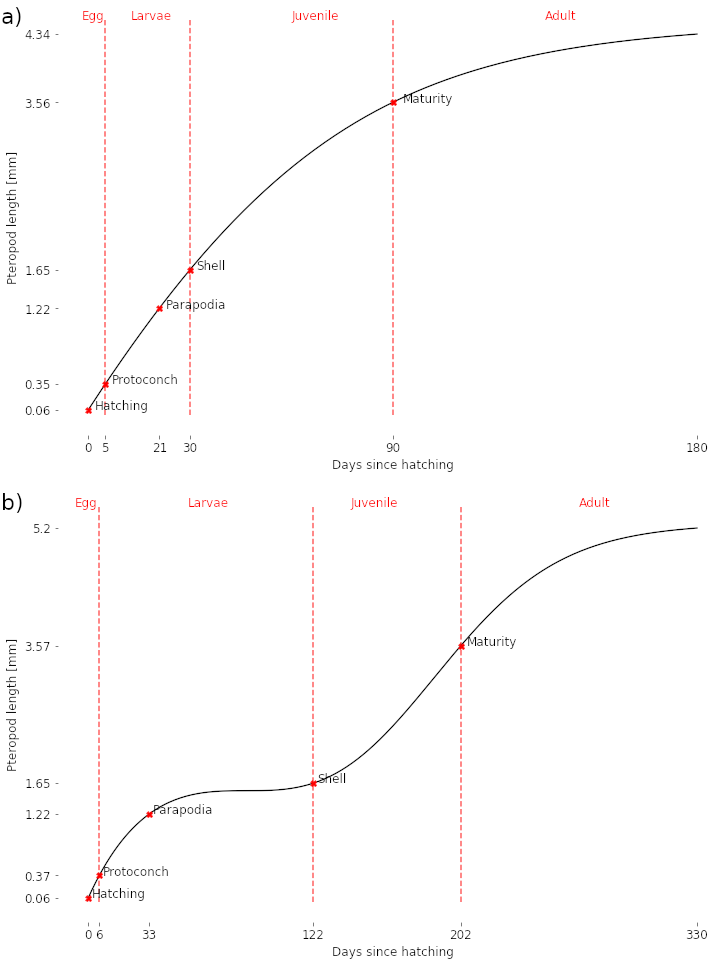
\includegraphics[scale=0.5]{images/Growth_both.png}
       
    
    \caption{Pteropod length growth (black line) calculated based on the growth rates described in \cite{Wang2017Lifecycle} for the (a) spring generation, and (b) the overwintering generation. The x-axis denotes the days since hatching. The y-axis denotes the length of the pteropod in mm. The red vertical lines separate the growth rate into the life stages, egg, larvae, juvenile, and adult. The red dots mark the hatching at day 0, and the development of key traits such as the protoconch (larval shell), parapodia (wings), shell, and maturity.}
    \label{fig:optimal_growth}
\end{figure*}


The duration of life stages and longevity of shelled pteropods under laboratory conditions \citep{Thabet2015Lifestages} matches with the longevity of pteropod populations between spring and summer in the field \citep{Wang2017Lifecycle}. However, for an overwintering pteropod population this is not the case. To determine the duration of life stages, we defined the shell length or organism length required for each pteropod to develop into the next stage using the developmental timings under laboratory conditions, and the length described by the growth function for the spring pteropod generation. Thus, the egg, larvae, and juvenile stages in both the spring and overwintering population last until they reach at least $0.35\,mm$, $1.65\, mm$, and $3.56\, mm$, respectively, and the parapodia are developed at a length of $1.22\,mm$ (Fig. \ref{fig:optimal_growth}).


\subsubsection{Calcification and dissolution of pteropod shells}

With the length thresholds for development between life stages of pteropods, and under the assumption that the growth function for spring and overwintering population presented above represent the growth of pteropods under optimal conditions, we can calculate the effect of dissolution on shell growth as a function of length and aragonite saturation state ($\Omega_{arag}$) in the environment. To this end, we calculate the loss of CaCO$_3$ or dissolution (in $mg$ CaCO$_3$) for a pteropod of length $L$ (in $mm$) that is exposed to a aragonite saturation state $\Omega_{arag}$. This is achieved by first calculating the shell mass $M$ in $mg$ CaCO$_3$ as a function of $L$ as presented in \cite{Bednarsek2014CalcificationDissolution}, which uses the conversion of shell length to dry weight \citep[DW; ][]{Bednarsek2012DryWeight}, the conversion of dry weight to total carbon \citep[0.25; ][]{Larson1986Carbon}, the fraction of particulate inorganic carbon in total carbon \citep[0.27; ][]{Bednarsek2012DryWeight}, and the molecular mass ratio of carbon to CaCO$_3$ \citep[8.33; ][]{Bednarsek2014CalcificationDissolution}. Second, we calculate the shell damage as percent shell loss per day ($V$) using the two-parameter exponential function fitted in \cite{Bednarsek2014CalcificationDissolution} for $\Omega_{arag}$ values ranging between $2.0$ and $0.6$ used in incubation experiments of pteropods of different sizes. Third, we multiply $V$ and $M$ to get the loss of CaCO$_3$:
\begin{eqnarray}
M & = & DW \cdot 0.25 \cdot 0.27 \cdot 8.33, \\
DW & = & 0.137 \cdot L^{1.5005}, \\
V & = & 65.75 \cdot e^{-4.7606 \cdot \Omega{arag}}, \\
loss & = & M \cdot V.
\end{eqnarray}


In addition to the dissolution, pteropods are able to repair their shells \citep{Bednarsek2014CalcificationDissolution}. Thus we also calculate the gain of CaCO$_3$ or calcification (in $mg$ CaCO$_3$) for a pteropod of length $L$ (in $mm$) that is exposed to a aragonite saturation state $\Omega_{arag}$. First, we calculate the rate of calcification ($Q$ in $\frac{\mu mol \, CaCO_3}{g Wet weight h}$) as presented in \citep{Comeau2010RepairRates}. Next, we calculate the wet weight of a pteropod with length $L$ \citep[$WW$ in $g$; ][]{Bednarsek2014CalcificationDissolution}. Finally, we multiply $Q$, $WW$, and the molar mass of CaCO$_3$ ($100.09 \frac{g}{mol}$) to get the gain of CaCO$_3$ in $\mu g$ CaCO$_3$ $h^{-1}$, which we transform to $mg$ CaCO$_3$ $d^{-1}$ and multiply by one day to match the units of the loss term mentioned in above:
\begin{eqnarray}
Q & = & 0.57 \cdot ln(\Omega_{arag}) + 0.25, \\
WW & = & \frac{DW}{0.28 \cdot 1'000}, \\
gain & = & Q \cdot WW \cdot 100.09 \cdot 1'000 \cdot 24 \cdot 1.
\end{eqnarray}
\noindent
The definition of the loss and gain terms as $mg$ CaCO$_3$ allows us to calculate the net effect of acidification on the shell growth, where after each day we calculate the deviation from the optimal shell growth defined for the spring and overwintering populations if the loss term exceeds the gain term. Additionally, since both calcification and dissolution are calculated as functions of $L$, our model takes the sensitivity of different stages into account, where early life stages are more sensitive to acidification relative to the adults (not shown, \textbf{preparing plot}).
Thus, using the size or shell length to define the transition between life stages, and the development of traits (e.g. parapodia, shell, maturity), we can simulate the net effect of acidification on the developmental timings of pteropod traits throughout their life, or the deviation from optimal growth.


\subsubsection{Diel vertical migration of pteropods}\label{sec:dvm}

A key morphological trait we defined in our IBM is the development of parapodia at a length of $1.22\,mm$ (Fig. \ref{fig:optimal_growth}), which in combination with the development of the aragonite shell allows pteropods to perform diel vertical migration (DVM). With the development of parapodia, pteropods counteract the negatively buoyant aragonite shell \citep{Byrne1984SettlingSpeed,Bergan2017SwimmingSinkingSpeeds} by swimming upwards in the water column \citep{Murphy2016UpwardSwimming}. The swimming speed of shelled pteropods varies between $13 \, mm \, s^{-1}$ for smaller pteropods and reaches $44\, mm\, s^{-1}$ for the largest ones \citep{Chang2012SwimmingSpeedSize}. We define $44\, mm\, s^{-1}$ as the maximum swimming speed of our pteropods, and approximate the effect of increasing size by multiplying the maximum swimming speed with the current shell length to maximum shell length $L_{\infty} = 5.31\, mm$ ratio (section \ref{sec:growthRates}). Thus, for a pteropod with $L = 1.6\,mm$ we model a swimming speed of roughly $13.3 \, mm \, s^{-1}$, which is within the range provided by \cite{Murphy2016UpwardSwimming} for pteropods with this shell length. Similarly, the sinking speed was modeled using a maximum terminal sinking speed of $18\, mm\, s^{-1}$ \citep{Bergan2017SwimmingSinkingSpeeds} and scaled with the current shell length to maximum shell length $L_{\infty}$ ratio, which takes into account the mass loss on settling velocity \citep{Byrne1984SettlingSpeed}.


In order to model DVM, we require the sinking depth, as well as the onset of the downward and upward migration. For the DVM depth, we use observations reported for the California Current System, where pteropods are mainly found in waters above $250\, m$ \citep{Bednarsek2015VerticalDistribution}. As was the case for the sinking and swimming speeds, the DVM depth increases with pteropod size, i.e. smaller pteropods are primarily located at the surface, and the largest ones sink to deeper layers  \citep{Bednarsek2015VerticalDistribution}. Thus, we chose a maximum DVM depth of $250\, m$ and calculate for each pteropod their maximum DVM depth by multiplying the maximum DVM depth with their current shell length to maximum shell length $L_{\infty}$ ratio. Finally, the onset of the downward and upward migration is taken from \cite{Bianchi2015GlobalDVM}, where pteropods start swimming downwards $21\, min$ before sunrise, and arrive at the surface from their maximum DVM depth $17\, min$ after sunset. 





\subsection{Physical module}

The physical module computes the advection and DVM of our pteropods using the Lagrangian ocean analysis tool Parcels v2.1.3 \citep{Delandmeter2019Unbeaching}. The ocean currents and environment surrounding out pteropods were taken from a basin-wide hindcast simulation with daily output of the aragonite saturation state, and the horizontal and vertical velocities  of the UCLA-ETH version of the Regional Oceanic Modeling System \citep[ROMS; ][]{shchepetkin2005regional} coupled with the biological elemental cycling model \citep[BEC; ][]{moore2013marine} for the period between 01/01/1979 and 31/12/2016. This hindcast simulation was done using a telescopic grid, which covers the Pacific Ocean basin with a horizontal grid spacing of $60$ $km$ that decreases to roughly $4$ $km$ towards central California \citep{frischknecht2018origin}. The refinement in horizontal resolution towards California properly simulates upwelling conditions along the California coastal region, and captures local \citep{frischknecht2018origin} as well as basin-wide processes \citep{frischknecht2015remote,frischknecht2017local}.

The advection was calculated using parcels built-in fourth-order Runge-Kutta integration scheme \citep{Delandmeter2019Unbeaching}. The integration uses a time step of one hour to calculate the position of the pteropods between two daily outputs. However, this advection scheme has been reported to result in beaching of particles \citep{Delandmeter2019Unbeaching}. Thus, as suggested in \cite{Delandmeter2019Unbeaching}, we implemented an artificial current that pushes our pteropods back to the ocean. Finally, we implemented a custom function to simulate DVM. The DVM function moves pteropods vertically according to their sinking and swimming speeds (section \ref{sec:dvm}). The DVM function uses the simulation time to check whether pteropods should be at the surface or at their maximum depth depending on the onset of the downward and upward migration. \textbf{Need to explain DVM function better!}

Apart from the movement of the pteropods, the physical module also keeps track of the environmental conditions that our pteropods experience each day. Thus, we implemented an $\Omega_{arag}$ tracker. The $\Omega_{arag}$ tracker calculates the average $\Omega_{arag}$ that each pteropod experienced each day during advection and DVM. The average $\Omega_{arag}$ is used in the population module to calculate the dissolution and calcification for each pteropod.


\subsection{Model setup and tuning}

The two components of our IBM model (populationa and physical modules) work in sequence. This means, that first the population module determines the mortality of each pteropod and determines the length, life stage, swimming, sinking, ERR index, time of downward and upward migration, and maximum depth for the surviving pteropods. Next the physical module runs for 24 hours, and calculates the advection, and DVM of each pteropod while keeping track of the $\Omega_{arag}$. Finally, the population module re-calculates the parameters mentioned before.


\begin{itemize}
    \item Problems with the model (e.g. drift from coast, re-seeding approaches,    
    \item Description of model tuning to the timing of abundance peaks as done for other IBMs \citep[e.g. ][]{Miller1998CalanusIBM}, and vertical distribution
    \item Model validation
\end{itemize}  

% \textbf{Need to read up on unbeaching functions used and reseeding approaches (Plankton zoonation problem!!)}
\subsection{Model evaluation}

The coupled physical-biological model uses the pteropod length to determine the life stage, and development of key traits (shell, parapodia, maturity). The growth in our IBM is simulated as a function of time and $\Omega_{arag}$. This model setup allows us to quantify the overall fitness of shelled pteropods. To this end, we use bulk quantities, such as the average shell size, CaCO$_3$ content, timing of abundance peaks, number of individuals reaching maturity, amount of dissolved CaCO$_3$, and the deviation from optimal growth.

    \begin{itemize}
        \item Case study of the bulk effect of acidification on shelled pteropods.
        \item Description of approach to separate between the effect of DVM, and life-stages in relation to acidification (i.e. advection-only model, no-DVM model, no-life-stages model, and full model). Spatiotemporal characterization
    
    \end{itemize}





% In the previous section \ref{sec:life_history_traits}, we presented the duration of the four stages used in our IBM. The combination of the stage duration with the length growth presented in section \ref{sec:physiological_traits} allows us to define the size required for each individual to develop into the next stage. Under optimal or spring conditions, the egg, larvae, and juvenile stages last until they reach $0.35\,mm$, $1.65\, mm$, and $3.56\, mm$, respectively (Fig. \ref{fig:optimal_growth}). 

% The stages of our IBM were defined based on the developmental timings of specific traits, such as the protoconch, and juvenile and adult shell (section \ref{sec:life_history_traits}). Both types of shells are susceptible to acidification with differing sensitivity \citep{Bednarsek2017ApplicationPteropodShell,Thabet2015Lifestages}. Such a definition allows us to characterize the calcification and dissolution rates for each pteropod at different stages of their life. To this end, we defined the calcification and dissolution rates as a function of the aragonite saturation state ($\Omega_{arag}$), as well as their shell length, were dissolution and calcification starts at the larvae stage.


% \textbf{Tons of equations here}




% the duration of the larvae stage is linked to the environmental conditions, such as temperature and food availability \citep{Paranjape1968egg,Hunt2008TopPredators,Gannefors2005Overwintering}.





% However, since shelled pteropods have shown a life stage specific sensitivity to changes in environmental condition \citep{Thabet2015Lifestages,Bednarsek2016CumulativeEffects}



% A longevity of six months
% Shelled pteropods have shown a life stage specific sensitivity to changes in environmental condition \citep{Thabet2015Lifestages,Bednarsek2016CumulativeEffects}. Thus, the shell growth rate described above was divided into four life stages in our IBM, i.e. into the egg, larvae, juvenile, and adult stage.



% The physiological traits simulated in the population model are the longevity, and growth rate. We use the longevity of temperate pteropod species as a basis for modeling the longevity of pteropods, due to the decreased influence of seasonal changes in environmental factors \citep[e.g. temperature and food availability; ][]{Bednarsek2012PteropodDistribution,Wang2017Lifecycle} on pteropod growth and longevity compared to polar species \citep{Manno2017ReviewPteropodVulnerability}. Under laboratory conditions the longevity of temperate \textit{Limacina retroversa} individuals was observed to be around six months \citep{Thabet2015Lifestages}. A similarly long longevity of six months is observed on the population level for \textit{L. helicina} during optimal growth conditions in spring in the temperate North Pacific \citep{Wang2017Lifecycle}. Thus, the pteropods in our IBM have a basis longevity of six months.

% The growth rates of shelled pteropods are taken from the three-year cohort analysis of the \textit{L. helicina} populations in the temperate North Pacific \citep{Wang2017Lifecycle}. \cite{Wang2017Lifecycle} provide the shell length ($L$) of pteropods as a function of time using measured length-frequency observations and a variation of the \textit{von Bertalanffy growth function} \citep[VBGF; ][]{Bertalanffy1938}, which considers seasonal changes ($S$) in growth rates. The formula used is as follows \citep{Somers1988,Wang2017Lifecycle}:
% \begin{eqnarray}
% L(t) & = & L_{\infty} \cdot (1 - e^{(K(t-t_0) + S(t) - S(t0))}), \\
% S(t) & = & \frac{CK}{2\pi} \cdot sin(2\pi (t-t_s)), \\
% t_s + 0.5 & = & WP,
% \end{eqnarray}
% \noindent
% where $L(t)$ denotes the length at age $t$, $L_{\infty}$ the maximum length, $K$ how fast $L_{\infty}$ is reached, $C$ the amplitude of growth oscillations, $t_0$ the age at $L=0$, $t_s$ the time between $t=0$ and the onset of oscillations in growth, and $WP$ the fraction of the year where growth is at its slowest. As was the case for the longevity, we use the growth function for the spring population as the basis growth function for our IBM (Fig. \ref{fig:optimal_growth}), where the values for $WP=0.1$ and $C=0.4$ where taken from \cite{Wang2017Lifecycle}. The values for $K=5.07\, s^{-1}$ and $L_{\infty} = 4.53\, mm$ are average values reported in \cite{Wang2017Lifecycle}.



% The duration of this stage is linked to the environmental conditions, such as temperature and food availability \citep{Paranjape1968egg,Hunt2008TopPredators,Gannefors2005Overwintering}, since it can undergo minimal to low growth in winter \citep[i.e. overwinter; ][]{Wang2017Lifecycle} and metamorphose to the juvenile stage in spring \citep{Hunt2008TopPredators}.






% Shelled pteropods have shown a  life stage specific sensitivity to changes in environmental condition \citep{Thabet2015Lifestages,Bednarsek2016CumulativeEffects}. Thus, the shell growth rate described above was divided into four life stages in our IBM, i.e. into the egg, larvae, juvenile, and adult stage. These four stages aggregate the ten-stage life cycle of the temperate pteropod \textit{Limacina retroversa} \citep{Howes2014Lab,Thabet2015Lifestages}. The transition between the stages is defined based on the timings of key traits such as the development of wings (parapodia), larval shell (protoconch), juvenile and adult shell, and maturity, since the aim of this study is to characterize the effects of acidification throughout the life of shelled pteropods that perform DVM. Thus, in combination with the shell growth rate described in the section \ref{sec:physiological_traits}, we define the size a pteropod needs to reach to transition between one stage to the next (Fig. \ref{fig:optimal_growth}).









% \textbf{Old version:}

% \subsection{Physiological traits} \label{sec:physiological_traits}
% The physiological traits simulated in the population model are the longevity, and growth rate. We use the longevity of temperate pteropod species as a basis for modeling the longevity of pteropods, due to the decreased influence of seasonal changes in environmental factors \citep[e.g. temperature and food availability; ][]{Bednarsek2012PteropodDistribution,Wang2017Lifecycle} on pteropod growth and longevity compared to polar species \citep{Manno2017ReviewPteropodVulnerability}. Under laboratory conditions the longevity of temperate \textit{Limacina retroversa} individuals was observed to be around six months \citep{Thabet2015Lifestages}. A similarly long longevity of six months is observed on the population level for \textit{L. helicina} during optimal growth conditions in spring in the temperate North Pacific \citep{Wang2017Lifecycle}. Thus, the pteropods in our IBM have a basis longevity of six months.

% The growth rates of shelled pteropods are taken from the three-year cohort analysis of the \textit{L. helicina} populations in the temperate North Pacific \citep{Wang2017Lifecycle}. \cite{Wang2017Lifecycle} provide the shell length ($L$) of pteropods as a function of time using measured length-frequency observations and a variation of the \textit{von Bertalanffy growth function} \citep[VBGF; ][]{Bertalanffy1938}, which considers seasonal changes ($S$) in growth rates. The formula used is as follows \citep{Somers1988,Wang2017Lifecycle}:
% \begin{eqnarray}
% L(t) & = & L_{\infty} \cdot (1 - e^{(K(t-t_0) + S(t) - S(t0))}), \\
% S(t) & = & \frac{CK}{2\pi} \cdot sin(2\pi (t-t_s)), \\
% t_s + 0.5 & = & WP,
% \end{eqnarray}
% \noindent
% where $L(t)$ denotes the length at age $t$, $L_{\infty}$ the maximum length, $K$ how fast $L_{\infty}$ is reached, $C$ the amplitude of growth oscillations, $t_0$ the age at $L=0$, $t_s$ the time between $t=0$ and the onset of oscillations in growth, and $WP$ the fraction of the year where growth is at its slowest. As was the case for the longevity, we use the growth function for the spring population as the basis growth function for our IBM (Fig. \ref{fig:optimal_growth}), where the values for $WP=0.1$ and $C=0.4$ where taken from \cite{Wang2017Lifecycle}. The values for $K=5.07\, s^{-1}$ and $L_{\infty} = 4.53\, mm$ are average values reported in \cite{Wang2017Lifecycle}.


% \begin{figure*}[tbh!]
%     \centering
    
%         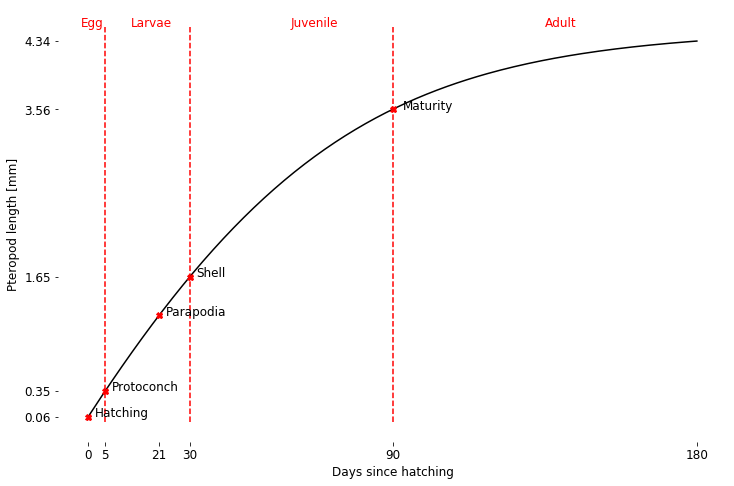
\includegraphics[scale=0.5]{images/Optimal_growth.png}
       
    
%     \caption{Pteropod length growth (black line) calculated based on the growth rates described in \cite{Wang2017Lifecycle}. The x-axis denotes the days since hatching. The y-axis denotes the length of the pteropod in mm. The red vertical lines separate the growth rate into the life stages, egg, larvae, juvenile, and adult. The red dots mark the hatching at day 0, and the development of key traits such as the protoconch (larval shell; day 5), parapodia (wings; day 21), shell (day 30), and maturity (day 90).}
%     \label{fig:optimal_growth}
% \end{figure*}


% \subsection{Life history traits}\label{sec:life_history_traits}

% Shelled pteropods have shown a  life stage specific sensitivity to changes in environmental condition \citep{Thabet2015Lifestages,Bednarsek2016CumulativeEffects}. Thus, the shell growth rate described above was divided into four life stages in our IBM, i.e. into the egg, larvae, juvenile, and adult stage. These four stages aggregate the ten-stage life cycle of the temperate pteropod \textit{Limacina retroversa} \citep{Howes2014Lab,Thabet2015Lifestages}. The transition between the stages is defined based on the timings of key traits such as the development of wings (parapodia), larval shell (protoconch), juvenile and adult shell, and maturity, since the aim of this study is to characterize the effects of acidification throughout the life of shelled pteropods that perform DVM. Thus, in combination with the shell growth rate described in the section \ref{sec:physiological_traits}, we define the size a pteropod needs to reach to transition between one stage to the next (Fig. \ref{fig:optimal_growth}).


% The egg stage lasts for five days. The egg stage summarizes all stages between spawning up to (but not including) the development of the protoconch \citep{Thabet2015Lifestages}. The larvae stage lasts for 25 days. This stage starts with the development of the protoconch, and includes the development of parapodia after roughly three weeks from spawning \citep{Thabet2015Lifestages}. The juvenile stage lasts for 60 days. This stage corresponds to the stage of rapid shell growth \citep{Thabet2015Lifestages}. Finally, the adult stage lasts for 90 days, and corresponds to the reproductive stage where pteropods develop female gonads \cite{lalli1989pelagic,Thabet2015Lifestages,Bednarsek2016CumulativeEffects}.


% The eggs of epipelagic shelled pteropod species are spawned as buoyant free-floating masses at the surface \citep{Lalli1978Reproduction,Paranjape1968egg,Schalk1990SeasonalSpatial,Gannefors2005Overwintering,Comeau2010Predation,Manno2016EggsAcidification}. While there is evidence for continuous low level spawning  throughout the year \citep{Wang2017Lifecycle,Thabet2015Lifestages}, pteropod  adults in a population have been found to have phases of synchronized widespread spawningm \citep[e.g. in spring and autumn][]{lalli1989pelagic,Thabet2015Lifestages,Wang2017Lifecycle}. During main spawning phases a pause of roughly 20 days has been observed between spawning of eggs \citep{Paranjape1968egg}. We modeled the time between spawning by defining a Egg Release Readiness Index (ERR), which is set to a random number between zero and one at maturation, increases by $\frac{1}{20}$ each day, and upon reaching $ERR \geq 1.0$ the eggs are released, and ERR is set to zero \citep[similar to the Clutch Readines Fraction presented in ][]{Miller1998CalanusIBM}.
% After the main spawning events adult pteropods have been observed to die \citep{Dadon1992Reproduction,Gannefors2005Overwintering,Hunt2008TopPredators,Howes2014Lab}.
% Resting stages

% The final life history trait we model in our IBM are the number of eggs produced by each individual. Upon reaching maturity, pteropod adults begin spawning eggs \citep{lalli1989pelagic,Gannefors2005Overwintering}. The number of eggs produced per reproductive pteropod adults has a high variability, ranging between $524$ and $10'051$ eggs (mean $5'936$) per \textit{L. helicina} female, and between $83$ and $650$ eggs (mean $260$) per \textit{L. retroversa} in a $20$ day period \citep{Lalli1978Reproduction}. This high variability in number of eggs is likely linked to the environmental conditions that pteropods experience \citep{Manno2016EggsAcidification}, since for instance reproductive \textit{L. helicina} adults produce between $465$ and $708$ eggs (mean $565$) over the 20 day period \citep{Paranjape1968egg}. As was the case for the physiological traits (section \ref{sec:physiological_traits}) we use the estimates for the warmer regions for our IBM, i.e. reproductive adults spawn $565$ eggs.


% \subsection{Morphological traits}

% In the previous section \ref{sec:life_history_traits}, we presented the duration of the four stages used in our IBM. The combination of the stage duration with the length growth presented in section \ref{sec:physiological_traits} allows us to define the size required for each individual to develop into the next stage. Under optimal or spring conditions, the egg, larvae, and juvenile stages last until they reach $0.35\,mm$, $1.65\, mm$, and $3.56\, mm$, respectively (Fig. \ref{fig:optimal_growth}). 

% The stages of our IBM were defined based on the developmental timings of specific traits, such as the protoconch, and juvenile and adult shell (section \ref{sec:life_history_traits}). Both types of shells are susceptible to acidification with differing sensitivity \citep{Bednarsek2017ApplicationPteropodShell,Thabet2015Lifestages}. Such a definition allows us to characterize the calcification and dissolution rates for each pteropod at different stages of their life. To this end, we defined the calcification and dissolution rates as a function of the aragonite saturation state ($\Omega_{arag}$), as well as their shell length, were dissolution and calcification starts at the larvae stage.


% \textbf{Tons of equations here}

% The final morphological trait we model in our IBM are the number of eggs produced by each individual. Upon reaching maturity, pteropod adults begin spawning eggs \citep{lalli1989pelagic,Gannefors2005Overwintering}. The number of eggs produced per reproductive pteropod adults has a high variability, ranging between $524$ and $10'051$ eggs (mean $5'936$) per \textit{L. helicina} female, and between $83$ and $650$ eggs (mean $260$) per \textit{L. retroversa} in a $20$ day period \citep{Lalli1978Reproduction}. This high variability in number of eggs is likely linked to the environmental conditions that pteropods experience \citep{Manno2016EggsAcidification}, since for instance reproductive \textit{L. helicina} adults produce between $465$ and $708$ eggs (mean $565$) over the 20 day period \citep{Paranjape1968egg}. As was the case for the physiological traits (section \ref{sec:physiological_traits}) we use the estimates for the warmer regions for our IBM, i.e. reproductive adults spawn $565$ eggs.



% \subsection{Behavioral traits}

% \textbf{Paragraph on motility, i.e. upward, downward swimming speed}

% \textbf{Paragraph on DVM, i.e. maximum depth, and timing}







\begin{table}[tbh!]
\caption{Summary of parameters used to model the physiological, life history, behavioral, and morphological traits of pteropods.}
\label{tab:parameters}
\begin{tabular}{l l}
\hline
\textbf{Parameter name}                          & \textbf{Parameter description}                                    \\ \hline
ID                                               & Unique identifier for each individual                    \\ 
Parent ID                                        & Unique identifier of parent individual                   \\ 
Parent shell size                                & Shell length of the parent pteropod at spawning                      \\ 
Generation                                       & Integer representation of the generation of individuals  \\ 
Life stage                                       & Integer representation of the life stage of the pteropod \\ 
Survive                                          & Boolean representation of survival                                 \\ 
Days since maturity                              & Number of days passed since maturity was reached                   \\ 
Days of growth                                   & Number of days the pteropod has grown                    \\ 
Egg release readiness (ERR)                      & \begin{tabular}[c]{@{}l@{}}Index between zero and one, which indicates\\ whether adult pteropods are ready to release \\ eggs ($ERR \geq 1.0$) or not ($ERR < 1.0$). \end{tabular}                                                         \\ 
Spawned                                          & \begin{tabular}[c]{@{}l@{}}Boolean representation of whether an adult \\ pteropod spawned eggs. \end{tabular}                                                        \\ 
Departure from depth                             & Time at which a pteropod swims towards the surface.                                                         \\ 
Departure from surface                           & Time at which a pteropod swims downwards.                                                                  \\ 
Up speed                                         & Upward swimming speed of a pteropod.                                                                  \\ 
Down speed                                       & Downward swimming speed of a pteropod                                                             \\ 
Maximum depth                                    & Maximum depth a pteropod can reach.                                                                  \\ 
Productivity                                     & \begin{tabular}[c]{@{}l@{}}Total phytoplankton productivity experienced \\ by a pteropod. \end{tabular}                                                                  \\ 
Sum of aragonite saturation state                & \begin{tabular}[c]{@{}l@{}}Sum of aragonite saturation state experienced \\ by a pteropod each day. \end{tabular}                                                                  \\ 
Number of intermittent steps                     &  Number of time steps used in the physical module.                                                                 \\ 
Depth of maximum chlorophyll a concentration     &  \begin{tabular}[c]{@{}l@{}}Depth at which a pteropod experienced \\ the maximum chlorophyll a concentration. \end{tabular}                                                                 \\ 
Longitude of maximum chlorophyll a concentration &  \begin{tabular}[c]{@{}l@{}}Longitude at which a pteropod experienced \\ the maximum chlorophyll a concentration. \end{tabular}                                                                  \\ 
Latitude of maximum chlorophyll a concentration  &   \begin{tabular}[c]{@{}l@{}}Latitude at which a pteropod experienced \\ the maximum chlorophyll a concentration. \end{tabular}                                                                \\ \hline
\end{tabular}
\end{table}




% \subsection{Physiological traits}
% The physiological traits simulated in the population model are the longevity, growth rate, and starvation tolerance of pteropods.

% The longevity and description of life stages for individual pterpods has been found to be around six months under laboratory conditions \citep[\textit{L. retroversa}; ][]{Thabet2015Lifestages}. This longevity of approximately six months for pteropods agrees with new findings on the longevity  of approximately six months in spring and eleven months for overwintering populations of \textit{L. helicina} observed in the temperate North Pacific \citep{Wang2017Lifecycle}.
% The longevity of six months for individual pteropods represents a longevity under optimal conditions. Thus, we used the population level longevity \citep[six and eleven months][]{Wang2017Lifecycle} to infer the longevity of individuals in our model. 

% The growth rate of shelled pteropods has been relatively uncertain \citep{Manno2017ReviewPteropodVulnerability}. However, the cohort analysis by \cite{Wang2017Lifecycle} revealed a strong seasonality, and dependence of the growth rate on temperature. The cohort analysis identifies an overwintering stage \citep{Wang2017Lifecycle}, which confirms previous observations of a veliger stage that overwinters before transitioning to a juvenile stage \citep{Paranjape1968egg,Gannefors2005Overwintering,Hunt2008TopPredators}, and thus extends the longevity of the pteropods to approximately eleven months in the temperate North Pacific. 


% The shell growth function uses a variation of the \textit{von Bertalanffy growth function} (VBGF), which considers seasonal changes in growth rates \citep{Somers1988,Wang2017Lifecycle}.


% \begin{itemize}
%     \item Maximum growth rate (Wang)
%     \item starvation tolerance (egg production despite starvation?) (search for this reference)
%     \item longevity (variable but some studies found around 6 months/11 months)(Wang, thabet, bednarsek)
% \end{itemize}

% \subsection{Life history traits}
% \begin{itemize}
%     \item Sexual reproduction
%     \item Reproduction frequency (Peranjape, clutch readiness)
%     \item Size at maturation (Wang)
%     \item resting stages (overwintering?) (Wang)
% \end{itemize}







% \textbf{OLD VERSION BELOW:}

% \subsection{physical module}




% (Check files to see the population drift at 31.Dec compared to initial population.

% \textbf{
% Need to read up on unbeaching functions used and reseeding approaches (Plankton zoonation problem!!). Also re-running population appears to have some problems on the main code! (does not compile, and dealing with no exposure does not work with the current implementations)}



% Subject of each section:
% \begin{itemize}
%     \item Description of pteropod IBM
%         \begin{itemize}
%             \item One subsection per module (population and particle module) \citep{Erguler2018Modules}
%             \item Description of the DVM kernel as a function of size \citep{Bianchi2013ImportanceDVM,Bednarsek2015VerticalDistribution,Murphy2016UpwardSwimming,Chang2012SwimmingSpeedSize,Byrne1984SettlingSpeed,Bergan2017SwimmingSinkingSpeeds}
%             \item Description of unbeaching function \citep{Delandmeter2019Unbeaching}
%             \item Description of exposure tracker \citep{Bednarsek2017ExposureHistory}
%             \item Description of mortality \citep{Bednarsek2016CumulativeEffects}
%             \item Problems with the model (e.g. drift from coast, re-seeding approaches, 
%         \end{itemize}
%     \item Description of model tuning to the timing of abundance peaks as done for other IBMs \citep[e.g. ][]{Miller1998CalanusIBM}, and vertical distribution
%     \item Description of ROMS hindcast simulation and using the CalCS as a case study
%     \item Model validation
    
    
%     \item Case study of the effect of acidification on shelled pteropods.
%     \begin{itemize}
%         \item Description of approach to separate between the effect of DVM, and life-stages in relation to acidification (i.e. advection-only model, no-DVM model, no-life-stages model, and full model)
        
%         \item Description of exposure metrics (e.g. average shell size, CaCO$_3$ content, timing of abundance peaks individuals reaching maturity, deviation from optimal growth function, amount of dissolved CaCO$_3$)
%     \end{itemize}
    
    
% \end{itemize}